%%
%% 研究報告用スイッチ
%% [techrep]
%%
%% 欧文表記無しのスイッチ(etitle,eabstractは任意)
%% [noauthor]
%%

%\documentclass[submit,techrep]{ipsj}
%%% <<< SES
%\documentclass[submit,techrep,noauthor]{ipsj}
% \documentclass[submit,ses,noauthor,dvipdfmx]{ipsj}
\documentclass[submit,noauthor,ses,dvipdfmx]{ipsj}
%%% >>> SES


\usepackage[dvips]{graphicx}
\usepackage{latexsym}
\usepackage{indentfirst}
\usepackage{url}	% \url{}コマンド用．URLを表示する際に便利
\usepackage{graphicx}  % ←graphicx.styを用いてEPSを取り込む場合有効にする
\usepackage{color}
\usepackage{listings}
\usepackage{multirow}
\usepackage{amsmath}
\usepackage{amssymb}
\usepackage{bm}
\usepackage{placeins}
\usepackage{float}
\usepackage{subcaption}
\usepackage{tabularx}
% \usepackage{caption} 

\renewcommand\lstlistingname{Program}
\newcommand{\todo}[1]{\colorbox{yellow}{{\bf TODO}:}{\color{red} {\textbf{[#1]}}}}
\newcommand{\done}[1]{\colorbox{green}{{\bf Done}:}{\color{black} {\textbf{[#1]}}}}
\newcommand{\memo}[1]{\colorbox{red}{{\bf memo}:}{\color{blue} {\textbf{[#1]}}}}
\newcommand{\fixstart}{\color{magenta}}
\newcommand{\fixend}{\color{black}}

\def\Underline{\setbox0\hbox\bgroup\let\\\endUnderline}
\def\endUnderline{\vphantom{y}\egroup\smash{\underline{\box0}}\\}
\def\|{\verb|}


\begin{document}
\raggedbottom


\title{OpenStackプロジェクトを対象に\\逆強化学習を用いた
モジュール別レビュー動態予測}


\affiliate{WU}{和歌山大学\\Wakayama University, Sakaedani 930, Wakayama-city 640--8510, Japan}


\author{橋本  一輝}{Hashimoto Kazuki}{WU}[s276189@wakayama-u.ac.jp]
\author{伊原  彰紀}{Ihara Akinori}{WU}[ihara@wakayama-u.ac.jp]

\vspace{-4mm}
\begin{abstract}
オープンソースソフトウェア (OSS) 開発において，将来的に開発者が数年単位で活動を継続するか否かを予測する手法が多数提案されている．従来研究の多くは，累積統計量を説明変数としてRandom Forest（RF）等の機械学習モデルを提案しているが，活動量の時系列的な変動を捉える手法は提案されていない．本研究は，特定のモジュールに対して特定の開発者が将来レビュー活動を行うか否かを予測（レビュー動態予測）するために，活動量の時系列的な変動に基づき学習する逆強化学習モデルを提案する．OpenStackのコードレビューに貢献する開発者436人を対象にケーススタディを実施したところ，RFと提案手法はほぼ同じAUC-ROCを示したが，両モデルは異なる開発者タイプの予測に成功する補完的な関係であることを明らかにした．
% 両モデルの単純平均によるアンサンブルは最良単独モデルに比べ$+2.2$パーセンテージポイントの改善を全評価期間で達成した．
% \todo{}OSSレビュアー継続予測では累積特徴量とRandom Forest（RF）が主流であり，行動の時系列パターンを直接扱う研究は限られていた．本研究は行動系列から報酬関数を推定するIRLをOpenStack 32リポジトリの4評価期間（1--3, 4--6, 7--9, 10--12か月）に適用し，RFと互角のAUCを示すこと，Archetypal Analysisで分解した開発者タイプ間でIRLとRFが補完的な得意領域を持つことを確認した．両モデル予測の単純平均によるアンサンブルは最良単独モデル比$+2.2$ パーセンテージポイントの改善を全評価期間で有意に達成した．
% \todo{従来研究では単一だったけど，本研究では32プロジェクトの活動を計測していることを示すか否か}
% \todo{活動と貢献の表記揺れ}
\end{abstract}

\maketitle
%%%%%%%%%%%%%%%%%%%%%%%%%%%%%%%

\section{はじめに}\label{sec:Introduction}
%%%%%%%%%%%%%%%%%%%%%%%%%%%%%%%

オープンソースソフトウェア (OSS) は，不特定多数の開発者からの貢献により支えられており，個人の知的好奇心や開発技術の学習などを動機として貢献している開発者も多い\cite{motivation}．Raymondらは，OSS開発の成功例としてLinuxプロジェクトを対象に調査し，不特定多数の開発者が自発的に参加する開発形態をバザール方式と呼ぶ\cite{bazzar}．
%この開発モデルは，多様な専門知識を有する開発者の参加を促進することで\todo{24時間開発・保守できるとか，もっといいことも書きたい}
この開発形態は，世界中の多様な専門知識を持つ開発者の参加を促進し，新規参入する開発者が増加する一方で，わずかな活動の後に活動を停止する開発者も多く，プロジェクト開発要員の流動性が極めて高い\cite{dynamics}．%また，開発者の参加動機が多様なため，時間的制約や興味の変化によって数回の活動後に活動を停止する開発者も多く，こうした
その結果，OSSプロジェクトの継続的な保守が困難になることもある\cite{pinto_otc}．

OSSの運用・保守は，長期間にわたりプロジェクトに貢献する一部の開発者（LTC: Long-Term Contributor) が担っていることが多く，このような開発者が活動を停止すると，実装方針，検証基準のような文書化されにくい知識の引き継ぎが困難になる．本研究で対象とするコードレビュー作業において，開発者の活動停止は，OSSの品質低下や特定モジュールを熟知する開発者の不足につながる\cite{bacchelli}\cite{mcintosh}．
したがって，将来的に発生する開発作業の依頼に対し，活動する開発者を確保できるかを見積もる手法が期待される．

% OSSプロジェクトの運用・保守は，長期貢献者 (Long-Term Contributor, LTC) など活動量や経験が一部のレビュアーに集中する構造で支えられている\cite{zhou}\cite{truckfactor}．
% こうしたレビュアーの離脱は単に人員の減少にとどまらず，設計判断の文脈や暗黙のレビュー基準といった文書化されにくい知識の喪失を招き，後続レビューの品質低下や特定領域でのレビュアー不足の発生につながる\cite{bacchelli}\cite{mcintosh}．
% 従来研究では，後継開発者の育成や開発知識の引き継ぎを計画的に進めるために，開発者の将来的な活動頻度や活動期間を事前に予測する手法が提案されている．\memo{引用３つの対応}\todo{XXらは，}開発者がプロジェクトへの貢献量（コミットやイシュー対応，等）に基づき，1年後以降や3年後以降に貢献しているか否かを予測する2クラス分類モデルを構築している
従来研究では，後継開発者の育成や開発知識の引き継ぎに向け，プロジェクトへの貢献量（コミット・イシュー対応等）に基づき1年後以降や3年後以降の開発者の活動継続を機械学習を用いて予測する2クラス分類モデルが提案されている\cite{zhou}\cite{bao}\cite{constantinou}．Shadeらは，ある特定の時点のコードレビュー依頼（以降，レビュー依頼）に，開発者が貢献するか否かを予測するモデルを構築している\cite{shade}．
% \todo{引用，コメントアウト見る}．
% %https://link.springer.com/article/10.1007/s10664-018-9646-1
これらの手法は，開発者のこれまでの累積統計量を用いて将来的な活動停止の有無を予測しているが，
リリースサイクルに同期した周期的な活動，集中的に取り扱うモジュールの変化，開発者の貢献停止，貢献再開など，時間的な変動を捉えられておらず，将来的に発生する特定モジュールに関する作業依頼に対し，貢献する開発者を確保できているか見積もる手法は提案していない．
% \todo{従来研究は，特定のプロジェクトの活動を学習している．．．って話はかけていないけど．．．．入れるか悩む}
% 累積活動量・採否率・直近性等を入力としたRandom Forest等の機械学習が主流であり，コミットやイシュー対応などプロジェクト全般の活動を貢献とみなして「N年後に継続しているか」を単一時点で二値予測することに留まっており，レビュー活動そのものへの継続的な参加に着目した研究は十分に進められていない\cite{zhou}\cite{bao}\cite{constantinou}．


% 加えて，レビュアー行動には，リリースサイクルに同期した周期的活動，コミット主体からレビュー専従への役割遷移，離脱と復帰の繰り返しといった時間的な変動があり，N年後の二値ラベルではこうした変動の情報が失われてしまう\cite{iaffaldano}．さらに入力側の累積特徴量も時間平均によって粒度が失われるため，こうした変動を捉えることが難しい．\todo{特定領域に特定の期間に依頼があったとき，誰かやってくれる人がいるかは，わからん．強化学習を使うと，やる/やらんの気配がわかるんじゃないか．}

% \todo{こうしたら問題を解決できるんじゃないかと考える}

本研究は，開発者への依頼と，開発者がその依頼に対して貢献したか否かを明確に観測できるレビュー活動を題材に，将来の開発者のレビュー動態（特定のモジュールに関するレビュー依頼に貢献するか否かの時間経過順の変化）を予測する逆強化学習モデルを提案する．具体的には，ある任意の時点で活動している開発者が，その先1年間を等期間に4分割し，それぞれの期間で特定のモジュールのレビュー依頼に貢献するか否かを予測するために，時系列情報を用いた逆強化学習モデルを用いる．



% 提案は次の3点からなる．
% \begin{itemize}
%     \item \textbf{複数の評価期間への予測対象分割}: 1--3, 4--6, 7--9, 10--12か月の4つの評価期間を予測対象とすることで，周期的活動や役割遷移などの時間変動を捉えることで，期間に応じて，必要リソースの事前見積もりや個別フォロー・依頼負荷調整（1--3か月），後継候補の育成（3--9か月），採用や領域別投資（10--12か月）といった対応策の検討が可能となる．
%     \item \textbf{開発者-ディレクトリペアでの予測}: 予測単位を開発者-ディレクトリペアとすることで，レビュー依頼の割り当てやディレクトリ単位での枯渇検知に直結する細粒度な情報が得られる．
%     \item \textbf{時系列符号化モデルIRLの採用}: 累積統計では捉えにくい行動の時間的変化を扱うため，行動系列から一貫した選好を報酬関数として推定する最大因果エントロピー逆強化学習（IRL）を採用する．
% \end{itemize}


% 以上の問題意識のもと，本研究では次の3つの研究設問（RQ）を立てる．
% \begin{itemize}
%     \item \textbf{RQ1}: 時系列符号化のIRLは累積特徴量のRFと比較してどれほど有効か．
%     \item \textbf{RQ2}: IRLとRFは開発者タイプによって予測の得意・不得意が分かれるか．
%     \item \textbf{RQ3}: 両モデルの統合により予測精度はどれほど向上するか．
% \end{itemize}

% \todo{貢献はあとで復活させるかもしれないけど，一旦コメントアウト}
% 本研究の貢献は次の3点である．第一に，OSSレビュアー継続予測に対しIRLを体系的に適用し，時系列符号化と累積統計ベースのRFを4つの評価期間で比較した．第二に，Archetypal Analysisをモデル得意領域の分析手法として導入し，開発者タイプ依存の補完性を複数の評価期間を横断して実証した．第三に，両モデルの予測確率を単純平均するアンサンブルを提案し，追加学習なしで有意な精度改善が得られることを示した．

本論文の構成は以下の通りである．\ref{sec:RelaatedWork}章で関連研究を整理し，本研究の位置付けを示す．\ref{sec:model}章で提案手法であるIRLモデルの構築方法，\ref{sec:evaluation}章で評価方法について述べる．\ref{sec:case}章でケーススタディを行い，\ref{sec:discuss}章で結果を考察する．\ref{sec:validity}章で妥当性への脅威を整理し，\ref{sec:conclusion}章で結論と今後の課題を述べる．

%%%%%%%%%%%%%%%%%%%%%%%%%
\section{関連研究}\label{sec:RelaatedWork}
%%%%%%%%%%%%%%%%%%%%%%%%%

\subsection{OSSプロジェクトに貢献する開発者の継続予測}
OSS開発者の継続性に関して多面的に調査されてきた．
Iaffaldanoらは一時的な活動休止の動機を分析し，私生活の出来事や興味の喪失といった個人要因と，プロジェクト貢献者間の対立やプロジェクト方針の変化といった組織要因から開発者が活動を停止することを示している\cite{iaffaldano}．Calefatoらはコア開発者の活動休止の頻度と復帰する確率を算出している\cite{calefato}．
Vasilescuらは性別および在籍期間の多様性がチームのメンバ入れ替わり率に与える影響を分析し，新規・熟練メンバが混在する度合いが高いチームほどメンバ入れ替わり率が高まる一方で，性別の多様性は入れ替わり率に有意な影響を示さないことを報告している\cite{vasilescu}．
% Vasilescuらは性別および在籍期間の多様性が離脱率に与える影響を分析し，性別の多様性は離脱率を低下させる一方で，在籍期間多様性\todo{在籍期間多様性ってどういう意味？いろんなタイミングで離脱してるって言ってるので，離脱率を増加させることと同義では？}は離脱率を増加させることを示している\cite{vasilescu}．
Linらは生存分析により，早期参加・ファイル修正中心・コーディング中心の活動パターンを持つ開発者ほど活動の継続期間が長いことを明らかにしている\cite{lin}．これらの従来研究では，開発者が多様な理由で貢献を継続・停止している知見を明らかにしており，事前に開発者の継続性を予測する手法の確立が期待される．

開発者の継続予測モデルを提案する従来研究では，将来の単一時点以降に開発へ貢献するか否かの2クラス分類モデルを提案している．
ZhouとMockusは，OSSプロジェクトへ新規に参加してから1か月間の累積活動量に基づき，1年後以降も継続して貢献するか否かを予測するモデルを構築した\cite{zhou}．BaoらはGitHubでアカウントを持つ開発者を対象に1年後，2年後，3年後以降に同じプロジェクトに貢献しているか否かを予測するモデルを構築している\cite{bao}．ConstantinouとMensは，RubyGems/npmエコシステムで規則性と長期継続の関連を示した\cite{constantinou}．Shadeらは，コードレビュー作業の依頼に，貢献する開発者を推薦する手法を提案している\cite{shade}．
% \todo{引用，コメントアウト見る}．
% %https://link.springer.com/article/10.1007/s10664-018-9646-1
これら従来研究では，リポジトリへのコミットやイシューに関する貢献の累積統計量を説明変数とした機械学習モデルを構築し，数年後の特定時点以降の活動の有無を予測するモデルを構築している．しかし，活動量の時系列的な変動（増減パターン）を捉える手法ではなく，将来のレビュー動態を数か月単位で予測する手法ではない．

% \subsection{タスク推薦・レビュアー推薦\todo{削除予定，}}
% 変更されたソースコードが要求を満たしているかを正確に判断できる開発者を特定するためのレビューア推薦手法が提案されている．Thongtanunamらは，変更されたソースコードと開発者のレビュー経験のあるソースコードを比較し，これらソースコードのファイルパス類似度に基づいてレビューアを推薦する手法を提案している\cite{thongtanunam}．YuらはGitHubのPull Requestに対する推薦をコードレビューとバグアサイン情報から構築した\cite{yu}．Rebaiらは多目的探索による推薦を提案している\cite{rebai}．ChouchenらはWhoReviewとして複数目的のレビュアー推薦アルゴリズムを提案している\cite{chouchen}．Shadeらは，コードレビュー作業の依頼に，貢献する開発者を推薦している．
% これらの従来研究は，推薦段階に最適化されており，推薦されたレビュアーが将来も継続して活動するかは明らかにしていない．

% レビュアー推薦は活発な研究分野である．Thongtanunamらはファイルパス類似度に基づくレビュアー推薦を提案している\cite{thongtanunam}．YuらはGitHubのPull Requestに対する推薦をコードレビューとバグアサイン情報から構築した\cite{yu}．Rebaiらは多目的探索による推薦を提案している\cite{rebai}．ChouchenらはWhoReviewとして複数目的のレビュアー推薦アルゴリズムを提案している\cite{chouchen}．これらは推薦段階に最適化されており，推薦されたレビュアーが将来も継続して活動するかは扱わない．

% \subsection{時系列モデルとIRLのOSSへの応用}
% 深層時系列モデルのOSS解析応用としては，HellendoornとDevanbuがソースコード生成でのLSTM等の有効性を比較している\cite{hellendoorn}．Vaswaniらが提案したTransformer以降，OSS解析でも応用が広がっている\cite{vaswani}．逆強化学習 (IRL) はNgとRussellによって始められた\cite{ng_russell}．Ziebartらは最大エントロピーIRL (MaxEnt IRL) を提案し，観測された行動軌跡を説明する報酬関数のうち，方策のエントロピーが最大となるものを推定する枠組みを確立した\cite{ziebart}．著者らの知る限り，OSSレビュアー継続予測へのIRL適用例は存在しない．

% \subsection{アンサンブル学習とArchetypal Analysis}
% アンサンブル学習はWolpertのStacked Generalizationを端緒として，誤りの直交性を活用して個別モデルを上回ることが知られている\cite{wolpert}．Archetypal AnalysisはCutlerとBreimanが導入したデータ表現手法である\cite{cutler_breiman}．MørupとHansenは機械学習・データマイニング応用を拡張した\cite{morup_hansen}．Eugsterはprofile可視化を提案した\cite{eugster}．本研究では，モデルの予測得意領域を分析する手法としてArchetypal Analysisを用いる．

% \subsection{本研究の位置付け\todo{この節もいらないかも}}
% 本研究は次の3点で既存研究と差別化される．第一に，OSSレビュアー継続予測を遠い単一時点ではなく1--3, 4--6, 7--9, 10--12か月の複数の評価期間で行い，複数時間粒度の予測を実証する．第二に，予測単位を開発者単独ではなく開発者-ディレクトリペアとし，レビュー依頼の割り当てやディレクトリ単位での枯渇検知に直結する細粒度な情報を扱う．第三に，行動系列から報酬関数を推定するIRLをOSSレビュアー継続予測に体系適用し，累積統計に基づくRandom Forestとの補完性をArchetypal Analysisで分析する．



\vspace{-2mm}
\section{逆強化学習を用いたモジュール別レビュー動態予測モデル}\label{sec:model}

本研究は，特定のモジュールに対して特定の開発者がレビューに貢献するか否かを予測する（レビュー動態予測）ために，ある任意の時点で活動している開発者の時間経過順の行動を捉えるモデルを構築する．なお，本研究ではモジュールをディレクトリ単位で定義し，以降ではディレクトリと表記する．具体的には，逆強化学習 (IRL: Inverse Reinforcement Learning) をレビュー動態予測に適用した手法を提案し，累積統計量に基づくRandom Forest (RF) と比較する．
% 通常のIRLは観察された行動の尤度を最大化する報酬関数を探索するが，観察されていない行動に対しては確率が0に近くなりやすく，開発者の多様な行動を適切に表現できない．そこで本研究では，観察された行動の特徴量を制約としつつ，未観測の行動の発生確率を0としないMCEを用いる．本手法により，過去に観察されていない行動に対しても有限の確率を割り当て，開発者行動の多様性を自然に表現した上で報酬関数を推定することが可能となる．\todo{MCEを書かないなら，「通常の」からここまでの文は削除かも}
具体的なモデル構築方法は\ref{sec:irl}項で述べる．
%図\ref{fig:model}は訓練期間・予測期間，図\ref{fig:label}は時間分割方法とラベルの付け方を示す．両図は本章で適宜参照する．


% 開発者が依頼を受け入れるか否かが明確に観測できるコードレビュー活動を題材に，将来のレビュー依頼に対する承諾可否を，開発者の行動変化を時間経過順に捉えるために強化学習モデルを提案する．具体的には，ある任意の時点で活動している開発者が，その先1年間を等期間に4分割し，それぞれの期間で特定のモジュールのコードレビュー依頼に貢献するか否かを予測するために，時系列符号化モデルIRを用いる．



% レビュー履歴から開発者-ディレクトリペアの状態系列と行動系列を構成し，IRLとRandom Forest（RF）が4評価期間（1--3, 4--6, 7--9, 10--12か月）の継続確率を独立に予測する．両モデルの予測確率の単純平均をアンサンブルとして最終出力とし，加えてArchetypal Analysisで分解した開発者タイプ別に両モデルの補完性を事後分析する．以下，\ref{sec:label-def}節で問題設定とラベル定義を述べ，次節以降で各構成要素を順に説明する．

\vspace{-4mm}
\subsection{強化学習・逆強化学習の基礎概念}

強化学習 (RL: Reinforcement Learning) は，エージェント（本研究では開発者）が環境に適応しながら将来にわたって得られる報酬の合計（累積報酬）の期待値を最大化する行動選択規則（以後，方策）を学習する枠組みであり，マルコフ決定過程に基づいて定式化される．逆強化学習 (IRL) は，RLを基本とする方法であるため，まずRLについて説明する．

RLは状態 $s$，行動 $a$，報酬関数 $r(s, a)$，方策 $\pi(a|s)$ の4つの要素から構成される．
状態はエージェントが観測する環境の情報，行動はエージェントが選択する操作，報酬関数は状態・行動の組に対して行動の良し悪しを数値で示す．方策は状態に対する行動の確率分布をそれぞれ表す．
ソフトウェア工学分野においても強化学習を適用した研究が進められており，Liuらはバグトリアージ問題にRLを適用し，バグレポートの情報を状態，開発者の選択を行動，割り当て結果の正否を報酬，どの開発者を選ぶかの行動選択規則を方策として定義している\cite{RL}．

通常，RLは報酬関数が既知であることを前提としている．
例えば，Liuらのバグトリアージでは，正しい開発者に割り当てたか否かという明確な基準を報酬関数として定義できる．しかし，本研究が対象とする開発者行動においては，レビュー依頼に対して貢献することが開発者にとって最良の選択であるかを事前に定義できない．したがって，本研究では開発者の行動パターンを正確に捉えるために，行動履歴から報酬関数を推定するIRLを用いる．
IRLは，エージェントの状態と行動の時系列記録である行動軌跡 $\tau$ を観察し，その行動を説明する報酬関数を逆算する枠組みである．
報酬関数 $r_\theta(s,a)$ は$n$次元の特徴量ベクトル $\phi(s, a)$ と学習により推定されるパラメータ（重みベクトル） $\theta$ の重み付き和$r_\theta(s,a) = \theta^\top \phi(s,a)$ として表現され，本研究では状態・行動の組に対する開発者の行動傾向を一つの数値で表す．
なお，$\theta$ の決定方法および推定した報酬関数から方策を導く方法については3.3.1項で述べる．

本研究では，開発者をエージェント，開発者が観測するレビュー活動の履歴を状態，特定のディレクトリのレビュー依頼に対する承諾・拒否を行動として定義する．
特徴量は開発者状態，ディレクトリ親和度，活動特徴の3カテゴリ37変数（詳細は3.2.1項の表\ref{tab:features}に示す）で構成し，IRLにより過去のレビュー行動履歴からレビュアーの暗黙的な判断基準を報酬関数として推定する．

\vspace{-2mm}
\subsection{特徴量・行動軌跡・ラベルの定義}\label{sec:label-def}
本研究では，開発者 $d$ とディレクトリ $r$ の組 $(d, r)$ を予測単位とし，図\ref{fig:model}に示すスナップショット時刻 $t_0$ における開発者の状態を起点とする．$t_0$ から遡る2年間（24か月）のレビュー履歴を月次に集約することで，$t_0$ 時点での開発者の状態を表現する．評価開始時点 $h \in \{0, 3, 6, 9\}$ ヶ月後を開始点とする3か月間を評価期間 $W_h$ とし，$W_h$内に受けたレビュー依頼に対して貢献するか否かを予測する．
% $t_0$ から $h$ か月後から3か月間を評価期間 $W_h$とし，$t_0$ 以前の訓練期間は$W_{\mathrm{train}}$ とする．
% スナップショット時刻を$t_0$とし，予測対象を開発者$d$とディレクトリ$r$の組$(d, r)$とする．

%----------------------
\begin{figure}[t]
\centering
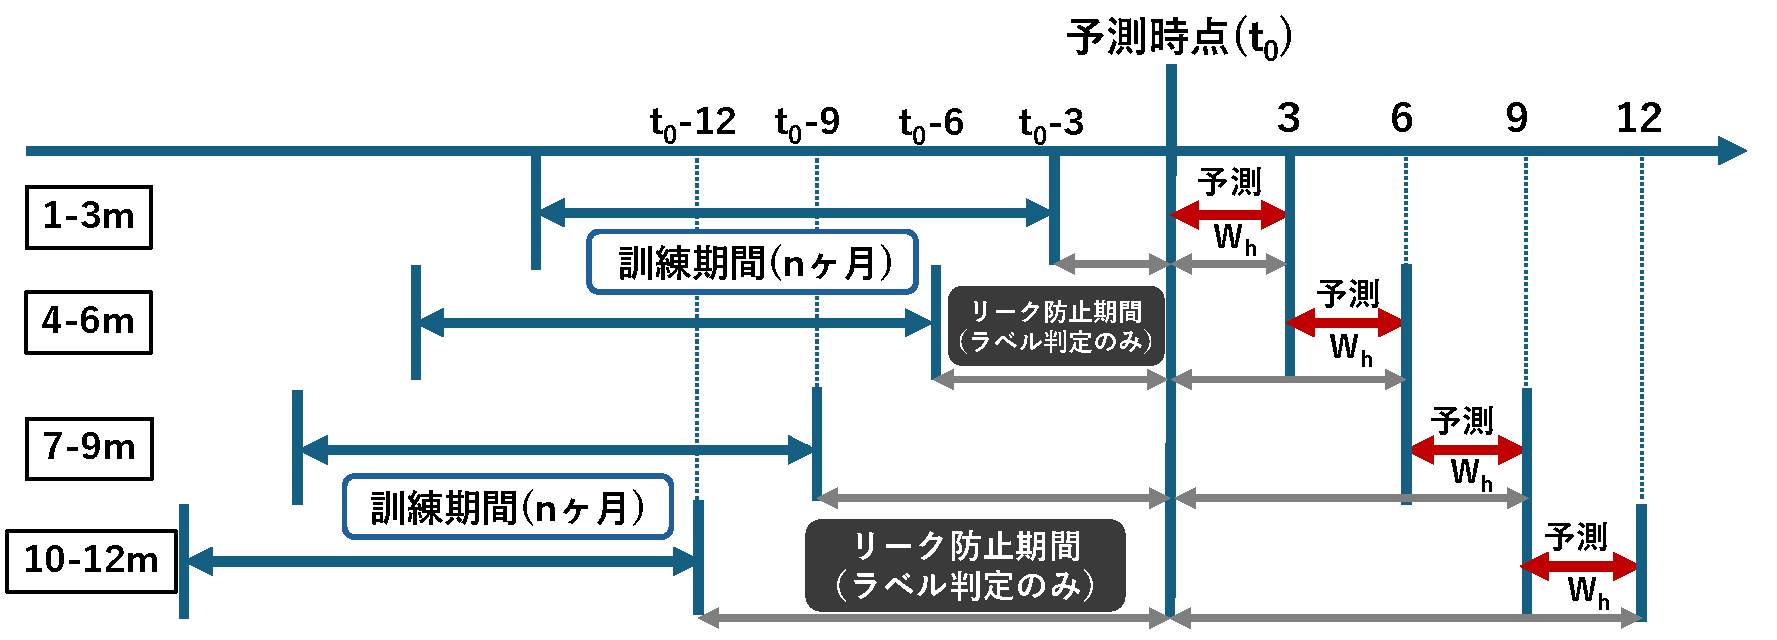
\includegraphics[width=\linewidth]{fig/fig_model.pdf}
\caption{各モデルの時間分割方法}
\label{fig:model}

\centering
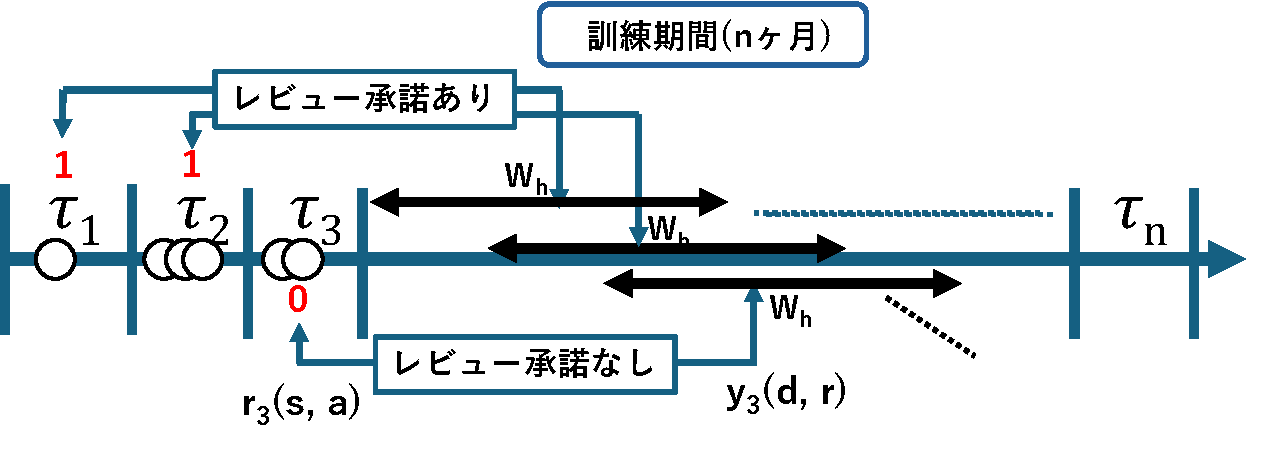
\includegraphics[width=\linewidth]{fig/fig_label3.pdf}
\caption{ラベル付の方法(例：1-3mモデル)}
\label{fig:label}
\end{figure}
%----------------------

\subsubsection{特徴量}
% 状態 $s \in \mathbb{R}^{32}$ は，開発者状態（26次元: 累積レビュー数・受諾率・直近性・揺らぎ指標等）とディレクトリ親和度（6次元: 当該ディレクトリでの過去レビュー数・直近性・受諾率・所有者重なり等）の合計32次元の特徴量で構成する．
% 行動を数値で表した行動特徴量 $\phi_a \in \mathbb{R}^5$ は，各月のレビュー行動を集計した5つの統計量（\todo{5次元の具体的な変数を書く}）を用いる．
% \todo{特徴量はリーク防止のため $[t_0 - W_{\mathrm{train}}, t_0]$ のみを参照する．}
% 状態$s \in \mathbb{R}^{32}$は，Random Forestモデルの構築でも使用するが，行動を表す$\phi_a \in \mathbb{R}^5$は，Random Forestモデルでは使用しない．


状態 $s$ は，表~\ref{tab:features} に示す通り，
開発者状態（26次元），ディレクトリ親和度（6次元），活動特徴（5次元）の計37次元から構成し，IRLとRFの両モデルで共通して使用する．なお，従来研究では評価対象のプロジェクト内の貢献のみを特徴量としているのに対し，本研究では分析対象とする他のプロジェクトへの貢献も特徴量として計測する．
% \todo{なお，未来情報の混入を防ぐため，特徴量の参照範囲は $[t_0 - W_{\mathrm{train}}, t_0]$ に限定する．}

%---------------------
\begin{table}[t]
\vspace{-4mm}
\caption{特徴量リスト}
\label{tab:features}
\centering
\begin{tabular}{p{1.7cm}rp{4.5cm}}
\hline
カテゴリ & 次元数 & 特徴量（抜粋） \\
\hline
開発者状態 & 26 & 累積レビュー数・受諾率・直近性・レビュー承諾/非承諾の変動回数等 \\
ディレクトリ親和度 & 6 & 過去レビュー数・直近性・受諾率・所有者重なり等 \\
活動特徴 & 5 & 活動の強度（レビュー行数，ファイル数）・応答速度・誰とレビューしたか\\
\hline
%合計 & 37 & \\
% \hline
\end{tabular}
\end{table}
%---------------------

\subsubsection{行動軌跡}

時刻 $t$ における1か月間の行動軌跡を $\tau_t = (s_t, \phi_{t}(s_t, a_t), y_t)$ と定義する．訓練軌跡 $\mathcal{T}$ は図~\ref{fig:label}に示すように，各月末を基準点として $\tau_t$ を時間経過順に集約することで，$\mathcal{T} = (\tau_1, \tau_2, \ldots, \tau_n)$ として訓練期間 $n$ か月の時系列として構成する．これにより，開発者の行動変化を時間経過順に捉えることが可能となる．
% なお，行動軌跡はIRLのみに使用し，RFでは使用しない．

\subsubsection{ラベル}
予測モデルの学習データのラベルとして，レビュー依頼に対して貢献するか否かのラベル $y_h(d, r)$ を図~\ref{fig:label}および式~(\ref{eq:label}) に示す通り定義する．
% \begin{equation}
% y_h(d, r) =\\
% \begin{cases}
% +1 & W_h\text{内に依頼あり \& 1件以上承諾} \\
% 0  & W_h\text{内に依頼あり \& 全拒否} \\
% 0^* & W_h\text{内に依頼なし，}t_0\text{から12か月以内に依頼あり} \\
% \text{除外} & \text{拡張期間にも依頼なし}
% \end{cases}
% \label{eq:label}
% \end{equation}
\vspace{-2mm} 
\begin{equation}
  y_h(d, r) =
  \vspace{-1mm} 
  \begin{cases}
  +1 & W_h\text{内に依頼あり かつ 1件以上貢献} \\
  0  & W_h\text{内に依頼あり かつ 貢献なし} \\
  0^* & W_h\text{内に依頼なし}
  \end{cases}
\label{eq:label}
\end{equation}

$0^*$ は弱負例として重み 0.5（正例・強負例は重み 1.0）を付与する．これはPU学習の考え方を踏襲し，依頼がない状態を強い負例として扱うと評価期間後半に貢献を再開する開発者を誤学習するため，判断できないケースを小さい重みで保持する~\cite{elkan_noto}．
学習に用いるラベルは月単位で，$W_h$ 内のレビュー依頼に対する承諾の有無に基づき付与する．

% 評価期間を$h \in \mathcal{H} = \{\text{1--3, 4--6, 7--9, 10--12か月}\}$の4つとし，$t_0$から見て$h$か月先の評価期間を$W_h$とする．これら4つの評価期間を合わせた$t_0$から12か月先までの期間を\textbf{拡張期間}と呼び，$W_h$内に活動がない場合の補助判定に用いる．継続フラグ$y_h(d, r)$を式(\ref{eq:label})に示す通り定義する．

% \begin{equation}
% \label{eq:label}
% y_h(d, r) = \begin{cases}
% +1 & W_h \text{内に依頼あり \& 1件以上承諾} \\
% 0 & W_h \text{内に依頼あり \& 全拒否} \\
% 0^{*} & W_h \text{内に依頼なし，拡張期間に依頼あり} \\
% \text{除外} & \text{拡張期間にも依頼なし}
% \end{cases}
% \end{equation}
% $0^{*}$は弱負例として重み0.1（正例・強負例は重み1.0）を付与する．これは正例・未ラベル（PU）学習の発想で，依頼が来ない状態を強い負例として扱うと評価期間後半に復活する開発者を誤学習するため，判断不能シグナルを小さい重みで保持する設計である\cite{elkan_noto}．

% ラベルは月単位で付与する．具体的には，各貢献日をその貢献月に紐づけ，月末を基準点として同一月内の全貢献に同じラベルを与える．基準点から$W_h$内のレビュー依頼に対する承諾の有無で$y_h$を判定する．予測対象は，開発者$d$がディレクトリ$r$において評価期間$W_h$内に1件以上のレビュー依頼を承諾する条件付き確率である．特徴量はリーク防止のため$[t_0 - W_{\mathrm{train}}, t_0]$のみを参照する．
\vspace{-2mm}
\subsection{モデル構築}

本節では，3.2節で定義した特徴量およびラベルを用いて構築する2つのモデルを説明する．\ref{sec:irl}項において，本研究で提案する時系列情報を用いて報酬関数を推定するIRLモデルについて述べる．\ref{sec:rf}項において，従来手法で頻繁に用いられる累積統計量から分類するRandom Forest (RF) モデルについて述べる．

\subsubsection{提案手法：IRLに基づくレビュー動態予測モデル}\label{sec:irl}

本節では，IRLのモデル構築手法として，報酬関数の定式化とLSTMを用いた特徴量ベクトルの計算，
および開発者が貢献する確率の推定方法を述べる．

報酬関数 $r_\theta(s,a) = \theta^\top \phi(s,a)$ を決定するために，観測された行動軌跡を説明しつつ，方策のエントロピーが最大となるパラメータ $\theta$ を求める．
ここで，過去のレビュー行動履歴の経験分布を $\mathcal{D}$ とすると，この問題は，過去のレビュー行動履歴から得られる報酬の期待値を最大化しつつ，方策の多様性を保つ次の最適化問題として定式化できる~\cite{ziebart}．
\begin{equation}
\max_\theta \mathbb{E}_{\mathcal{T} \sim \mathcal{D}}
\left[\sum_t r_\theta(s_t, a_t)\right] - \log Z(\theta)
\label{eq:mce}
\end{equation}
ここで，$\mathbb{E}_{\mathcal{T} \sim \mathcal{D}}[\cdot]$ は過去のレビュー行動履歴 $\mathcal{D}$ から得られた行動軌跡 $\mathcal{T}$ に対する期待値を表す．
また，$Z(\theta)$ は方策の確率分布の合計が1になるよう調整する正規化定数であり，$-\log Z(\theta)$ は方策のエントロピーを最大化する．エントロピーを最大化することで，未観測の行動に対しても有限の確率を割り当てることができる．

式~(\ref{eq:mce}) を解くと，方策は$\pi_\theta(a|s) \propto \exp(r_\theta(s,a))$ の形，すなわちsoftmax関数として表現される．softmax関数は，貢献する確率として $[0, 1]$ で出力する．
学習パラメータ $\theta$ の更新には最適化アルゴリズムであるAdam\cite{adam}を用い，cross-entropyを損失関数として最小化する（学習率 $= 3\times10^{-4}$，エポック数 $= 150$，乱数シード $= 777$）．
なお，検証データの損失が15エポック改善しない場合に学習を早期終了する．
%Kingma, D. P. and Ba, J.: Adam: A Method for Stochastic Optimization, arXiv:1412.6980 (2014).




% 3.1節で述べた通り，通常のIRLは観察された行動の尤度を最大化する報酬関数を探索するため，未観測の行動に対しては確率が0になりやすい．本研究では，MCEのアルゴリズムに基づき，観察された行動の特徴量を制約としつつ，未観測の行動の発生確率を0としない．

% 報酬関数 $r_\theta(s,a)$ は，3.1節での述べた通り，パラメータ $\theta$ を用いた特徴量ベクトル $\phi(s,a)$ との重み付き和 $r_\theta(s,a) = \theta^\top \phi(s,a)$ として表現する．ここで $\phi(s,a)$ は状態系列をLSTM（hidden dim $= 128$, 1層）で
% 月次処理した際の最終hidden stateである．


% 観測された行動軌跡を説明する報酬関数のうち，
% 方策のエントロピーが最大となるものを求める問題は，
% 次の二重問題に帰着する~\cite{ziebart2008}．
% \begin{equation}
% \max_\theta \mathbb{E}_{\tau \sim \pi_E}
% \left[\sum_t r_\theta(s_t, a_t)\right] - \log Z(\theta)
% \label{eq:mce}
% \end{equation}
% 双対形 $\pi_\theta(a|s) \propto \exp(r_\theta(s,a))$ はsoftmax形をとり，
% その負の対数尤度はsoftmax cross-entropyとして表現できる．






% 状態 $s$ は開発者状態（26次元: 累積レビュー数・受諾率・直近性・揺らぎ指標等）とディレクトリ親和度（6次元: 当該ディレクトリでの過去レビュー数・直近性・受諾率・所有者重なり等）からなり，行動特徴$\phi_a$は当該月のレビュー行動の集約統計を用いる．訓練軌跡は各月末を基準点として状態$s_t$と行動特徴$\phi_a^t$を集約し，\ref{sec:label-def}節のラベル付け規則を各月末に適用して$y_t$を得ることで，軌跡$\tau = (s_t, \phi_a^t, y_t)_{t=1}^T$が訓練期間$T$か月の時系列として構成される．専門家方策$\pi_E$は軌跡集合の経験分布として与える．

% 報酬を$r_\theta(s, a) = \theta^\top \phi(s, a)$と線形パラメータ化（$\phi$はLSTM hidden state）し，観測された行動軌跡を説明する報酬関数のうち，方策のエントロピーが最大となるものを求める問題は，次の二重問題に帰着する\cite{ziebart}．
% \begin{equation}
% \label{eq:mceirl}
% \max_\theta \mathbb{E}_{\tau \sim \pi_E}\left[\sum_t r_\theta(s_t, a_t)\right] - \log Z(\theta)
% \end{equation}
% 双対形$\pi_\theta(a \mid s) \propto \exp(r_\theta(s, a))$はsoftmax形をとり，その負の対数尤度はsoftmax cross-entropyとして表現できる．

% 状態系列をLSTM（hidden dim = 128, 1層）で月次処理し，最終hidden stateを$\phi$とする線形ヘッドで報酬$r_\theta(s_T, a)$を求めたうえで，継続行動に対するsoftmax確率を継続スコア$\hat{p}^{\mathrm{irl}}(d, r) \in [0, 1]$として出力する\cite{hochreiter_lstm}．学習はAdamで負の対数尤度を最小化する
% \todo{学習率とか入れるか考える}（lr = $3 \times 10^{-4}$，EPOCHS = 150，early stopping patience = 15，SEED = 777）．

\subsubsection{比較手法：Random Forestを用いたレビュー貢献予測モデル}\label{sec:rf}
本研究では，比較対象として従来研究で使用されることの多いRandom Forest (RF) を用いたモデルを構築する．RFは複数の決定木を組み合わせた学習手法であり，各決定木の予測結果の多数決により最終的な予測を行う．
本研究では，3.2節で定義した37次元の特徴量を用いて学習する\cite{breiman_rf}．貢献する確率は $[0, 1]$ で出力する．学習設定には，決定木の数$= 100$，乱数シード$=777$ を用いる．

%%%%%%%%%%%%%%%%%%%%%%%%%%%%%
\section{評価方法}\label{sec:evaluation}
%%%%%%%%%%%%%%%%%%%%%%%%%%%%%

\subsection{予測精度の評価方法}
本研究の予測単位は開発者-ディレクトリのペア $(d, r)$ であり，評価もこのペアを基本単位（ペア単位）とする．ただし，積極的に活動する開発者が多くのディレクトリに関わっている場合，その開発者の行動結果が評価に大きく影響するため，開発者ごとに集計した単位（開発者単位）の評価結果も示す．予測精度の評価指標として，ペア単位および開発者単位の両方にAUC-ROCを用いる．AUC-ROCは，モデルが貢献する開発者と貢献しない開発者をどれだけ正しく識別できるかを$[0, 1]$の数値で表す指標であり，1に近いほど予測精度が高いことを示す．

% 本章では，IRLとRFの予測精度を比較するための評価方法を述べる．
% 具体的には，評価指標と統計検定，およびIRLとRFのそれぞれが予測可能な開発者の特徴を明らかにするために原型分析を行うため，その分析方法を述べる．

% \subsection{評価指標と統計検定}

% 本研究の予測単位は開発者-ディレクトリのペア $(d, r)$ であり，評価もこのペアを基本単位（ペア単位）とする．ただし，積極的に活動する開発者が多くのディレクトリに関わっている場合，
% その開発者の行動結果が評価に大きく影響するため，開発者ごとに集計した単位（開発者単位）の評価結果も示す．

% 予測精度の評価指標として，ペア単位および開発者単位の両方にAUC-ROCを用いる．
% AUC-ROCは，モデルが貢献する開発者と貢献しない開発者をどれだけ正しく識別できるかを$[0, 1]$の数値で表す指標であり，1に近いほど予測精度が高いことを示す．




% (i) IRL単独，(ii) RF単独，(iii) アンサンブル（提案）の3種を比較する．ペア単位の指標としてAUC-ROC（bootstrap 95\%信頼期間付き）を，開発者単位の指標として開発者別AUCを併用する．開発者別AUCに対する2つの比較（アンサンブル vs IRL，アンサンブル vs RF）で paired Wilcoxon 符号順位検定（両側）を行い，Bonferroni 補正（補正係数 2）を適用する．効果量は rank-biserial $r$ で示す．

% なおペアレベルのbootstrapは同一開発者が複数ペアを持つ場合の開発者内相関を無視するため，95\%信頼期間を楽観側に評価する可能性がある．補完として開発者別AUCに対するWilcoxon検定を併用し，開発者単位での頑健性を確認する．


\subsection{モデルが予測できるペア・開発者の分析方法}

本研究では，IRLとRFのそれぞれが予測可能な開発者の特徴を明らかにするために原型分析を行う．
原型分析は，データ中の極端なパターン（原型）を複数用意し，対象のデータ点がどの原型に近いかを表現する手法である~\cite{cutler_breiman}．

本研究では，予測実験と同様に，開発者-ディレクトリのペア $(d, r)$ を単位とするペア単位と，開発者ごとに集計した開発者単位の2つの粒度で原型分析を行う．原型分析で対象とする原型数は，原型数を増やしても平均残差平方和の改善が小さくなる点に基づき選択する．なお，原型分析は予測には用いず，IRLとRFの両モデルが予測可能な開発者の特徴を明らかにする手法として位置付ける．


% 両モデルの得意・不得意領域を解釈するため，$t_0$直前6か月の特徴量集計期間内にレビュー・PR履歴がある開発者を対象にArchetypal Analysisを適用する\cite{cutler_breiman}．凸制約付きALSにより学習し，原型数$K$はRSS/Nのelbowで選択する．各開発者は$K$原型上の重み$\alpha \in \Delta^{K-1}$で表現し，主帰属を$\arg\max \alpha$で割り当てる．archetypeは予測には用いず，両モデルの補完性を事後的に分析する手法として位置付ける．


%%%%%%%%%%%%%%%%%%%%%%%%%%%%%
\section{ケーススタディ}\label{sec:case}
%%%%%%%%%%%%%%%%%%%%%%%%%%%%%

\subsection{実験設定}

\noindent\textbf{対象リポジトリ：}評価対象はOpenStackの公式サービスリポジトリ33件のうち，分析対象期間にレビュー履歴が存在しなかったsunbeamを除く32リポジトリとする．なお，特徴量の計測においては，評価対象のリポジトリだけでなく，開発者が貢献する他のリポジトリへの活動も計測対象に含める．

% ===== 査読対応 A-6 ここから =====
\fixstart
OpenStackを評価対象として選定した理由は次の3点である．第一に，コードレビュー管理システムGerritにより，レビュー依頼・応答が構造化されたログとして取得できることである．第二に，governanceに登録されたサービスチームを単位として，本研究が前提とする「リポジトリ内ディレクトリ」という粒度でモジュールを一貫して定義できる32件の主要リポジトリを客観的な基準で選定できることである．第三に，OpenStackは開発者の継続予測に関する既存研究\cite{zhou}\cite{bao}\cite{constantinou}でも対象とされてきた代表的な大規模OSSであり，先行研究との比較可能性が高いことである．Gerritを用いる大規模OSSとしてはAndroid Open Source Project (AOSP) 等も存在するが，AOSPはリポジトリの名前空間の深さが不均一でチーム単位のリポジトリ選定が難しく，本研究では見送った．
\fixend
% ===== 査読対応 A-6 ここまで =====

% \subsection{データセットと前処理}
\noindent\textbf{データ取得と前処理：}
% 評価対象はOpenStack governanceに登録された33のservice teamの代表リポジトリのうち，sunbeamを除く32リポジトリとする．
OpenStackプロジェクトではコードレビュー管理システムGerritを使用している．Gerritでは任意のコードレビュー依頼1件につき1つのチケットが作成され，レビュアーの指定，議論，ソースコードの承認などが管理される．各チケットにはレビュー依頼した開発者を列挙したreviewersフィールドがあり，本研究ではこのフィールドから依頼された開発者を取得する．
ただし，reviewersフィールドに登録されていないが，レビューに貢献した開発者も存在するため，reviewersフィールドの開発者とレビューに貢献した開発者の和集合をレビュー依頼の対象とする．
% なお，依頼したレビュアーのメールアドレスからbotアカウント（CI/CD等）を対象外とするために，\todo{XX}とのパターンマッチで自動的に特定する．
% 全データをレビュー依頼時刻でソートする．
% なお，依頼したレビュアーのメールアドレスからbotアカウント（CI/CD等）を\todo{何との？パターンマッチということはXとYのパターンを比較するってことですよね？}パターンマッチにより除外する．

% また，レビュー依頼に対して開発者が貢献した履歴は，Gerrit REST API\footnote{\url{https://review.opendev.org/}}によって，著者らが2024年10月にデータ収集するまでの履歴を取得し，，レビュー依頼した開発者がレビュー対象のソースコードに対して承認，要修正，コメントのいずれかの応答を行ったか否かを2値ラベルとして取得する．\todo{「レビューの依頼時刻は，作成時刻とする」と書きたい？}タイムスタンプにはチケットの作成時刻を用いる．
なお，依頼されたレビュアーのうちbotアカウント（CI・自動化）は除外する．具体的には，Gerritアカウントのユーザ名またはメールアドレスに，CI・自動化アカウントを示す部分文字列（\texttt{zuul}，\texttt{gerrit}，\texttt{-ci-}，\texttt{-test@}，\texttt{-bot@}，\texttt{@review.openstack.org} 等）が含まれるかを部分一致で判定し，該当するアカウントを除外する．

また，レビュー依頼に対して開発者が貢献した履歴は，Gerrit REST API\footnote{\url{https://review.opendev.org/}}を用いて，レビュー依頼した開発者がレビュー対象のソースコードに対して承認，要修正，コメントのいずれかの応答を行ったか否かを2値ラベルとして取得する．各レビュー依頼の時刻（レビュー依頼時刻）には，チケットの作成時刻を用いる．

\noindent\textbf{時間分割：}
評価対象の開始時点$t_0$は，2023年01月01日00時00分00秒とし，訓練期間は3年間，評価期間は1年間とする．なお，$t_0$を単一時点に固定しているため，異なる時点での再現性は未検証であり，妥当性への脅威として7章で議論する．

\noindent\textbf{データセットの規模：}
訓練期間と評価期間の両方で観測される$(d, r)$ペア$n = 4,534$（436開発者）を分析対象とする．
また，原型分析は$t_0$直前6か月にレビュー・実装履歴がある289開発者のペア$n = 3,747$に限定する．

\vspace{-2mm}
\subsection{予測モデルの評価結果}

% 本節の主指標はペア単位AUC-ROCであり，主結果は$n = 4{,}534$ペアから算出する．
表~\ref{tab:rq1}と表~\ref{tab:rq1-1}は，それぞれ開発者-ディレクトリのペア単位と開発者単位のIRLとRFのAUC-ROCの結果を示す．各表では4つの評価期間を区別して示す．
ペア単位における両モデルのAUC-ROCの絶対値差は[0.1-5.2]パーセンテージポイント (以下，pp) 以内に収まり，開発者単位の両モデルAUC-ROCの絶対値差は[0.9-4.6]であった．全体としてRFが上回る傾向ではあるが，IRLはRFと大きな精度差は見られなかった．
次節で両モデルが予測できる開発者の特徴を分析する．


% \todo{以降RQをなくす}
% \subsection{RQ1: 時系列符号化のIRLは累積特徴量のRFと比較してどれほど有効か}

\begin{table}[h]
\centering
\caption{開発者-ディレクトリペア単位AUC-ROC（$n=4{,}534$）}
\label{tab:rq1}
\begin{tabularx}{\linewidth}{l*{3}{>{\centering\arraybackslash}X}}
\hline
評価期間 & IRL & RF & IRL$-$RF (pp) \\
\hline
1--3か月  & 0.826 & 0.791 & $+3.5$ \\
4--6か月  & 0.813 & 0.812 & $+0.1$ \\
7--9か月  & 0.751 & 0.792 & $-4.1$ \\
10--12か月 & 0.754 & 0.806 & $-5.2$ \\
\hline
4期間平均 & \textbf{0.786} & \textbf{0.800} & $\mathbf{-1.4}$ \\
\hline
\end{tabularx}

\centering
\caption{開発者単位AUC-ROC（$N=436$)}
\label{tab:rq1-1}
\begin{tabularx}{\linewidth}{l*{3}{>{\centering\arraybackslash}X}}
\hline
評価期間 & IRL & RF & IRL$-$RF (pp) \\
\hline
1--3か月  & 0.873 & 0.882 & $-0.9$ \\
4--6か月  & 0.861 & 0.872 & $-1.1$ \\
7--9か月  & 0.826 & 0.871 & $\mathbf{-4.5}$ \\
10--12か月 & 0.805 & 0.851 & $\mathbf{-4.6}$ \\
\hline
4期間平均 & 0.841 & \textbf{0.869} & $\mathbf{-2.8}$ \\
\hline
\end{tabularx}
\end{table}

%----------------------
% \begin{table}[t]
% \centering
% \caption{開発者-ディレクトリペア単位AUC（$n=4{,}534$）\todo{差し替えと文章の修正}}
% \label{tab:rq1}
% \begin{tabularx}{\linewidth}{l*{3}{>{\centering\arraybackslash}X}}
% \hline
% 評価期間 & IRL & RF & IRL$-$RF (pp) \\
% \hline
% 1--3か月 & 0.779 & 0.792 & $-1.4$ \\
% 4--6か月 & 0.770 & 0.804 & $-3.4$ \\
% 7--9か月 & 0.774 & 0.789 & $-1.5$ \\
% 10--12か月 & 0.779 & 0.793 & $-1.3$ \\
% \hline
% 4期間平均 & \textbf{0.775} & \textbf{0.794} & $\mathbf{-1.9}$ \\
% \hline
% \end{tabularx}



% \centering
% \caption{開発者単位AUC（$N=xxx$）\todo{差し替えと文章の修正}}
% \label{tab:rq1-1}
% \begin{tabularx}{\linewidth}{l*{3}{>{\centering\arraybackslash}X}}
% \hline
% 評価期間 & IRL & RF & IRL$-$RF (pp) \\
% \hline
% 1--3か月  & XXXXX & XXXXX & $XXXX$ \\
% 4--6か月  & XXXXX & XXXXX & $XXXX$ \\
% 7--9か月  & XXXXX & XXXXX & $XXXX$ \\
% 10--12か月 & XXXXX & XXXXX & $XXXX$ \\
% \hline
% 4期間平均 & \textbf{XXXXX} & \textbf{XXXXX} & $\mathbf{XXXX}$ \\
% \hline
% \end{tabularx}
% \end{table}
%----------------------




% 表\ref{tab:rq1}に開発者-ディレクトリペア単位AUCを4評価期間で示す．両予測モデルの差は$\pm 4$ pp以内に収まり，時系列符号化のIRLは累積特徴量のRFとほぼ互角の精度を達成し，IRLでも従来手法と同等の予測が可能であることを確認した．時系列符号化単独で予測精度を底上げするのは限界があるが，全体精度が同等であっても両モデルが異なる開発者を正しく当てている可能性が残るため，次節で補完性の有無を検証する．
% \FloatBarrier
\vspace{-2mm}
\subsection{モデルが予測できるペア・開発者の分析結果}
本節では，4章で述べた原型分析を用いて，IRLとRFのそれぞれが予測できる
開発者-ディレクトリのペアおよび開発者の特徴を分析する．分析対象は$t_0$直前6か月にレビューや実装履歴を持つ開発者289人，およびそれらに関与するペア$n = 3,747$ペアに限定する．図\ref{fig:rss}は，原型数$K$に対する平均残差平方和の推移を示す．原型数$k=3$から$k=4$で平均残差平方和が大きく改善し$k=5$以降は改善幅が小さくなったため$K=4$を採用する．

%---------------------
\begin{figure}[t]
\centering
\begin{minipage}[t]{0.48\linewidth}
\centering
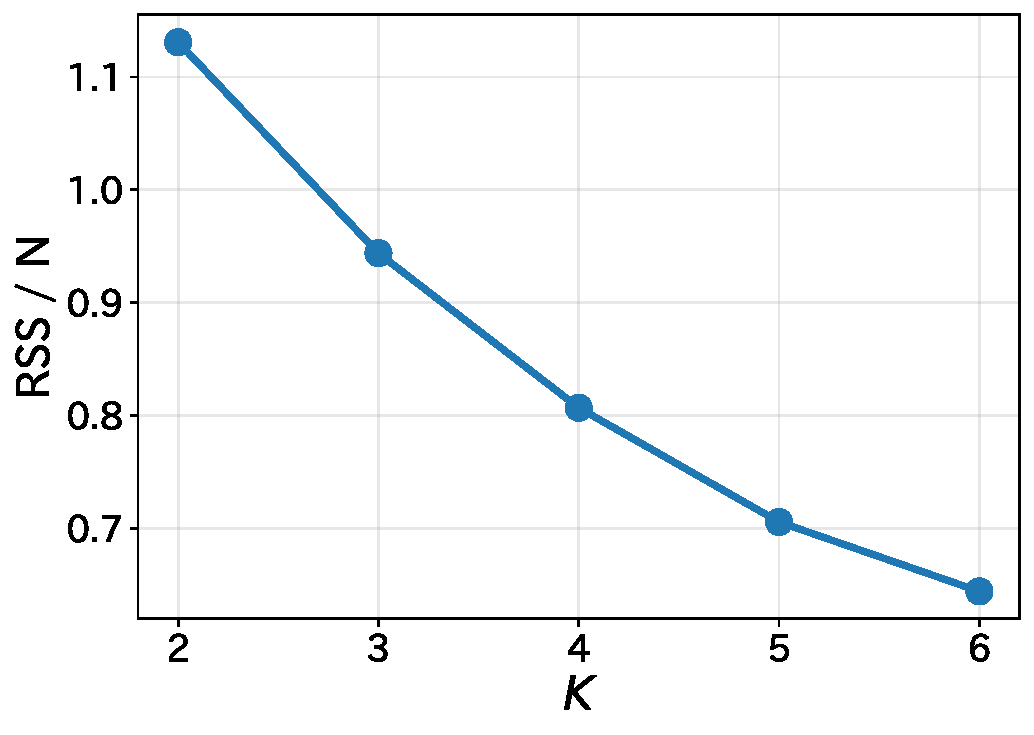
\includegraphics[width=\linewidth]{fig/fig_pair_elbow.pdf}
\subcaption{ペア単位（$n=3{,}677$）}
\label{fig:pair-elbow}
\end{minipage}
\hfill
\begin{minipage}[t]{0.48\linewidth}
\centering
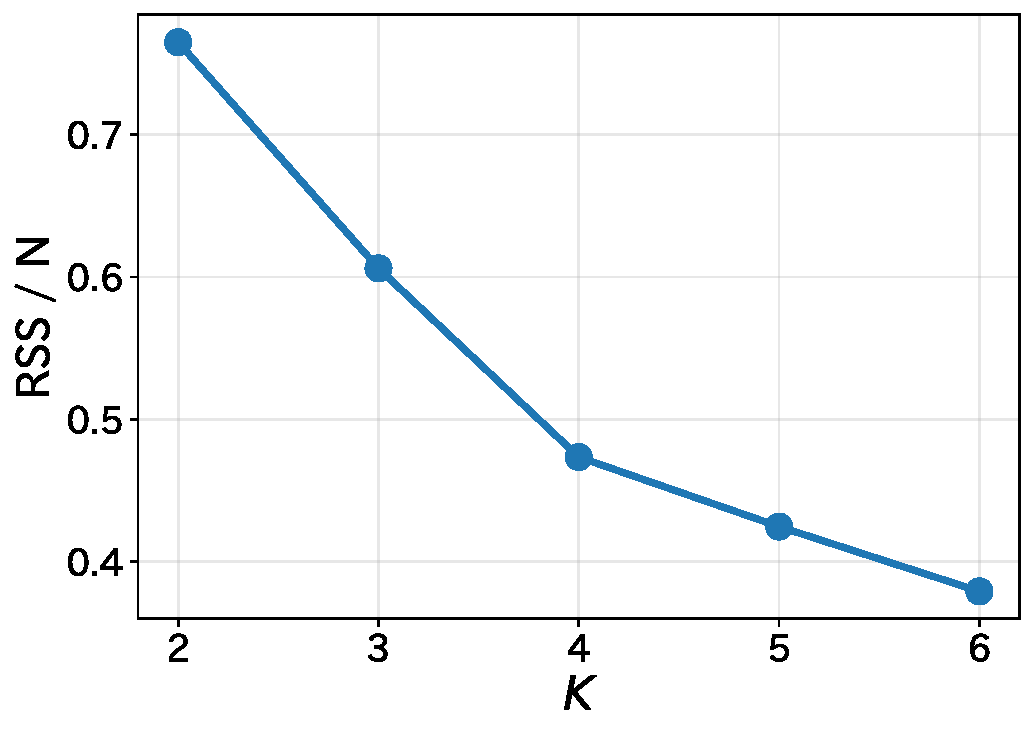
\includegraphics[width=\linewidth]{fig/fig_dev_elbow.pdf}
\subcaption{開発者単位（$N=289$）}
\label{fig:dev-elbow}
\end{minipage}
\caption{原型数$K$に対する平均残差平方和の推移．}
\label{fig:rss}
\vspace{-4mm} 
\end{figure}
%------------------


\subsubsection{ペア単位の分析}\label{sec:pair-arch}

% \todo{リリースサイクルに同期した周期的な活動，集中的に取り扱うモジュールの変化，開発者の貢献停止，貢献再開のあたりの議論は？}
ペア単位の原型分析では，開発者とディレクトリを単位として分類する．特徴量は表\ref{tab:features}に示す37個の特徴量を用いる．
% 図~\ref{fig:rss}(a)により$K = 4$を採用し，
表~\ref{tab:pair-arch}と図~\ref{fig:pair-profile}は，原型分析によって設定した4つの原型の解釈名，および，それぞれの原型の特徴量の分布を示す．表~\ref{tab:pair-arch}に示す特徴の列は，図~\ref{fig:pair-profile}の分析結果をまとめている．図~\ref{fig:pair-profile}の横軸は他の原型の平均との差，縦軸は特徴量名を示す．

表~\ref{tab:pair-arch-delta}にペア単位の4原型における評価期間別のAUC差（IRL$-$RF）を示す．
P1（他プロジェクト経験者）では4期間中3期間でIRLの方が精度が高く，当該ディレクトリへの貢献経験が少ないペアでは，時系列情報を考慮したIRLが有効である．
P2（関与低下型）では短期（1--3か月）においてのみIRLがやや優位であり，中長期ではRFが上回る．これは関与低下の初期段階における活動パターンの変化を時系列モデルが捉えることができたためと考える．
P3（高承諾型）では，短期を除いて概ねRFが優位であり，累積レビュー実績が豊富な開発者-ディレクトリペアに対しては累積統計量を用いたRFが有効である．
P4（低活動・低承諾型）では全期間にわたってRFが優位であり，活動が疎なペアではIRLの学習に十分な行動軌跡が得られなかったことが理由と考える．

したがって，特定のディレクトリへの貢献経験が少ないペアではIRLが，貢献経験が豊富なペアではRFが有効であることを示した．特に，最も多くのペアを含むP1（$n = 1{,}284$）においてIRLが優位であることは，提案手法の有効性を示す重要な結果である．

% したがって，ディレクトリ経験が薄い領域ではIRLの時系列推論が，経験が厚い領域ではRFの累積統計量が有用であることを示した．


% ペアarchetypeは開発者とディレクトリの関係性を分類する．特徴量はstate 26次元とpath特徴量6次元の計32次元を用いる．得られた4原型の解釈名と$n$を表\ref{tab:pair-arch}に，特徴量プロファイルを図\ref{fig:pair-profile}に示す．

% \begin{table}[H]
% \centering
% \caption{4 ペアarchetype の解釈名（$n=3{,}677$）}
% \label{tab:pair-arch}
% \begin{tabularx}{\linewidth}{l|l|X|r}
% \hline
% ID & 名前 & 特徴 & $n$ \\
% \hline
% P1 & 他プロジェクト経験者 & 開発者はactiveだが当該ディレクトリ経験ほぼなし & 1{,}284 \\
% P2 & 関与低下型 & ディレクトリ経験あり，承諾率は極低 & 928 \\
% P3 & 高承諾型 & ディレクトリ経験豊富，承諾優位 & 539 \\
% P4 & 低活動・低承諾型  & 開発者・ディレクトリとも中程度の関与 & 926 \\
% \hline
% \end{tabularx}
% \end{table}

% \begin{figure}[H]
% \centering
% 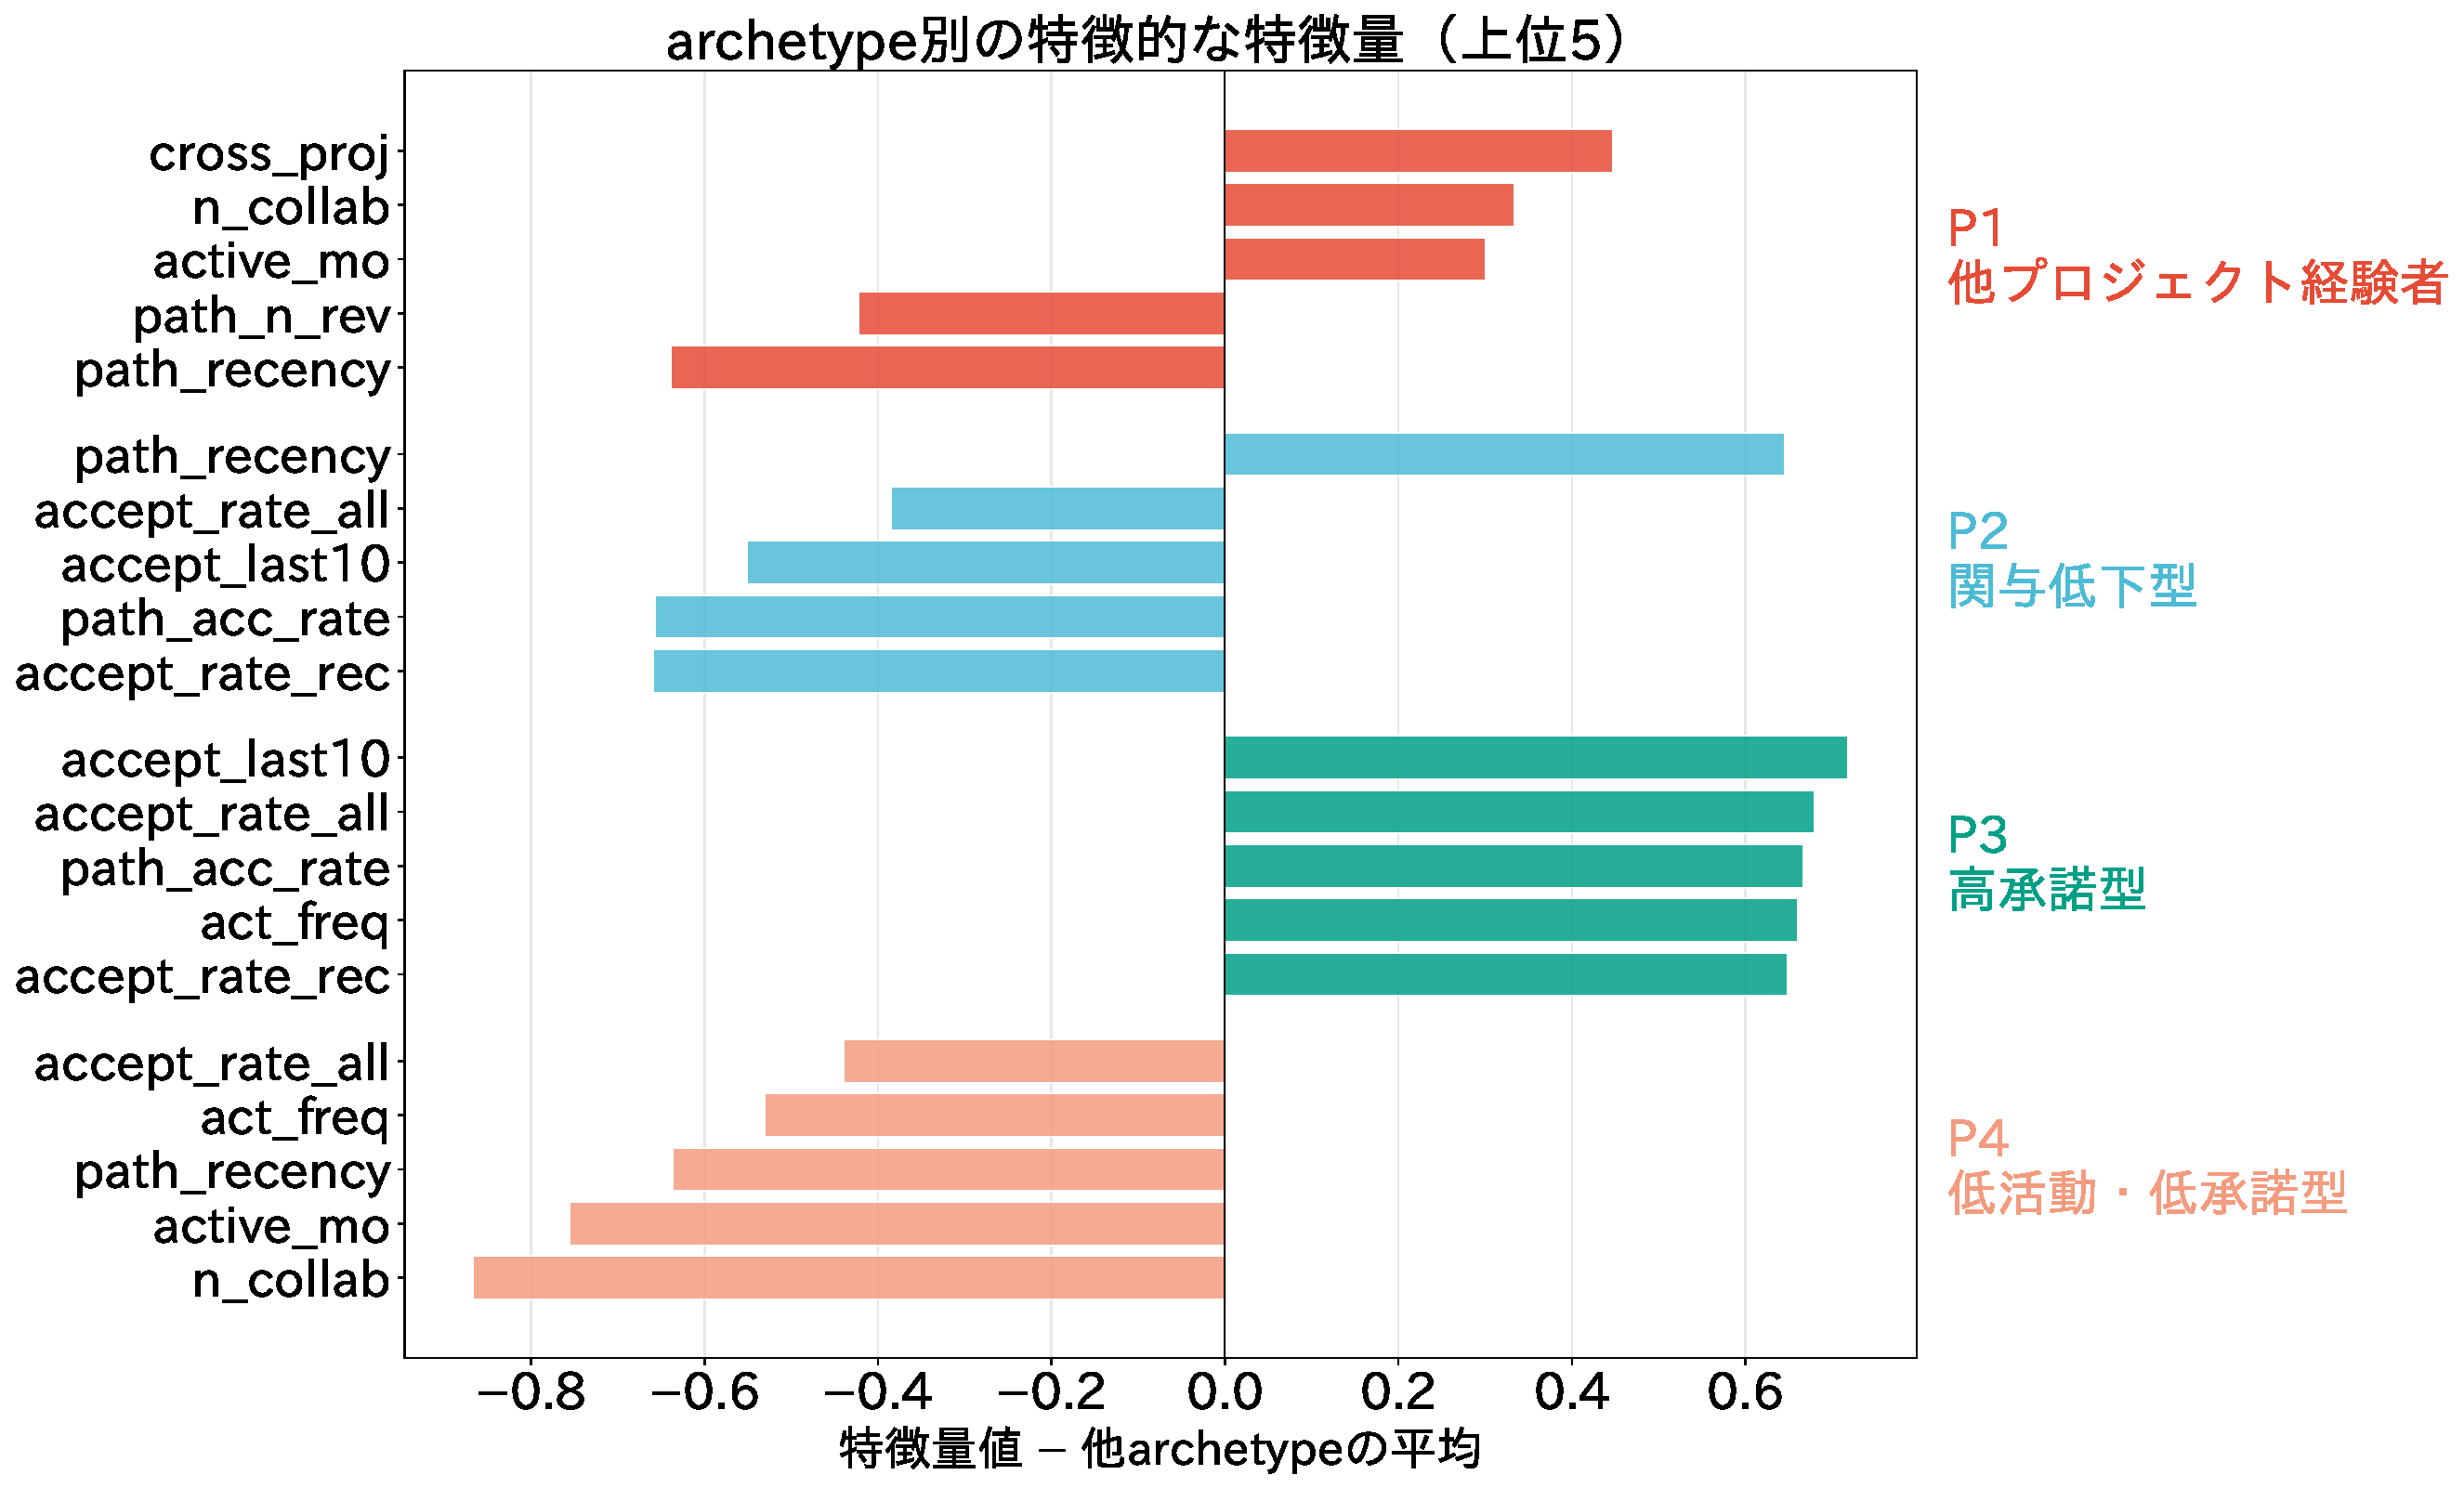
\includegraphics[width=\linewidth]{fig/fig_pair_archetype_profile.pdf}
% \caption{4 ペアarchetypeの特徴的な特徴量（他archetype平均との差，上位5）．}
% \label{fig:pair-profile}
% \end{figure}

% \subsubsection{ペアタイプ別の補完性}
% 表\ref{tab:pair-arch-delta}にペアarchetype $\times$ 評価期間のAUC差（IRL$-$RF）を示す．\textbf{P1（他プロジェクト経験者）ではIRL優位}（4期間中3期間で正），\textbf{P2（関与低下型）とP3（高承諾型）ではRF優位}（全体に負），\textbf{P4（低活動・低承諾型 ）では混在}という構造が観察される．ディレクトリ経験が薄い領域ではIRLの時系列推論が，経験が厚い領域ではRFの累積統計が効きやすいと解釈できる．

% \begin{table}[H]
% \centering
% \caption{ペアarchetype $\times$ 評価期間のAUC差 IRL$-$RF（pp，$n=3{,}677$）\todo{差し替え}}
% \label{tab:pair-arch-delta}
% \small
% \begin{tabularx}{\linewidth}{l|*{4}{>{\centering\arraybackslash}X}}
% \hline
% Arch. ($n$) & 1--3m & 4--6m & 7--9m & 10--12m \\
% \hline
% P1 (1,284) & $+5.7$ & $+0.1$ & $+6.9$ & $-1.6$ \\
% P2 (928) & $-7.6$ & $-6.1$ & $-3.3$ & $-4.9$ \\
% P3 (539) & $-8.9$ & $-8.9$ & $+1.1$ & $-1.3$ \\
% P4 (926) & $+4.1$ & $-1.9$ & $-3.9$ & $+2.9$ \\
% \hline
% \end{tabularx}
% \end{table}

% \begin{figure*}[t]
% \centering
% \begin{minipage}[t]{0.48\linewidth}
%   % 右列：ペア単位
%   \begin{table}[H]
%   \centering
%   \caption{4 ペアarchetype の解釈名（$n=3{,}677$）}
%   \label{tab:pair-arch}
%   \begin{tabularx}{\linewidth}{l|p{1.5cm}|X|r}
%   \hline
%   ID & 名前 & 特徴 & $n$ \\
%   \hline
%   P1 & 他プロジェクト経験者 & 他プロジェクトへの貢献経験（cross\_proj）を有し，最終活動からの経過時間（path\_recency）が短いが，ディレクトリへの過去レビュー数（path\_n\_rev）は少ない & 1{,}284 \\
%   P2 & 関与低下型 & 最終活動からの経過時間（path\_recency）が長く，承諾率（accept\_rate\_all等）が低い & 928 \\
%   P3 & 高承諾型 & 承諾率（accept\_rate\_all等）が高い & 539 \\
%   P4 & 低活動・低承諾型  & 全体承諾率（accept\_rate\_all）が低く，活動頻度（act\_freq）も少ない & 926 \\
%   \hline
%   \end{tabularx}
%   \end{table}

% \vspace{-8mm}

%   \begin{figure}[H]
%   \centering
%   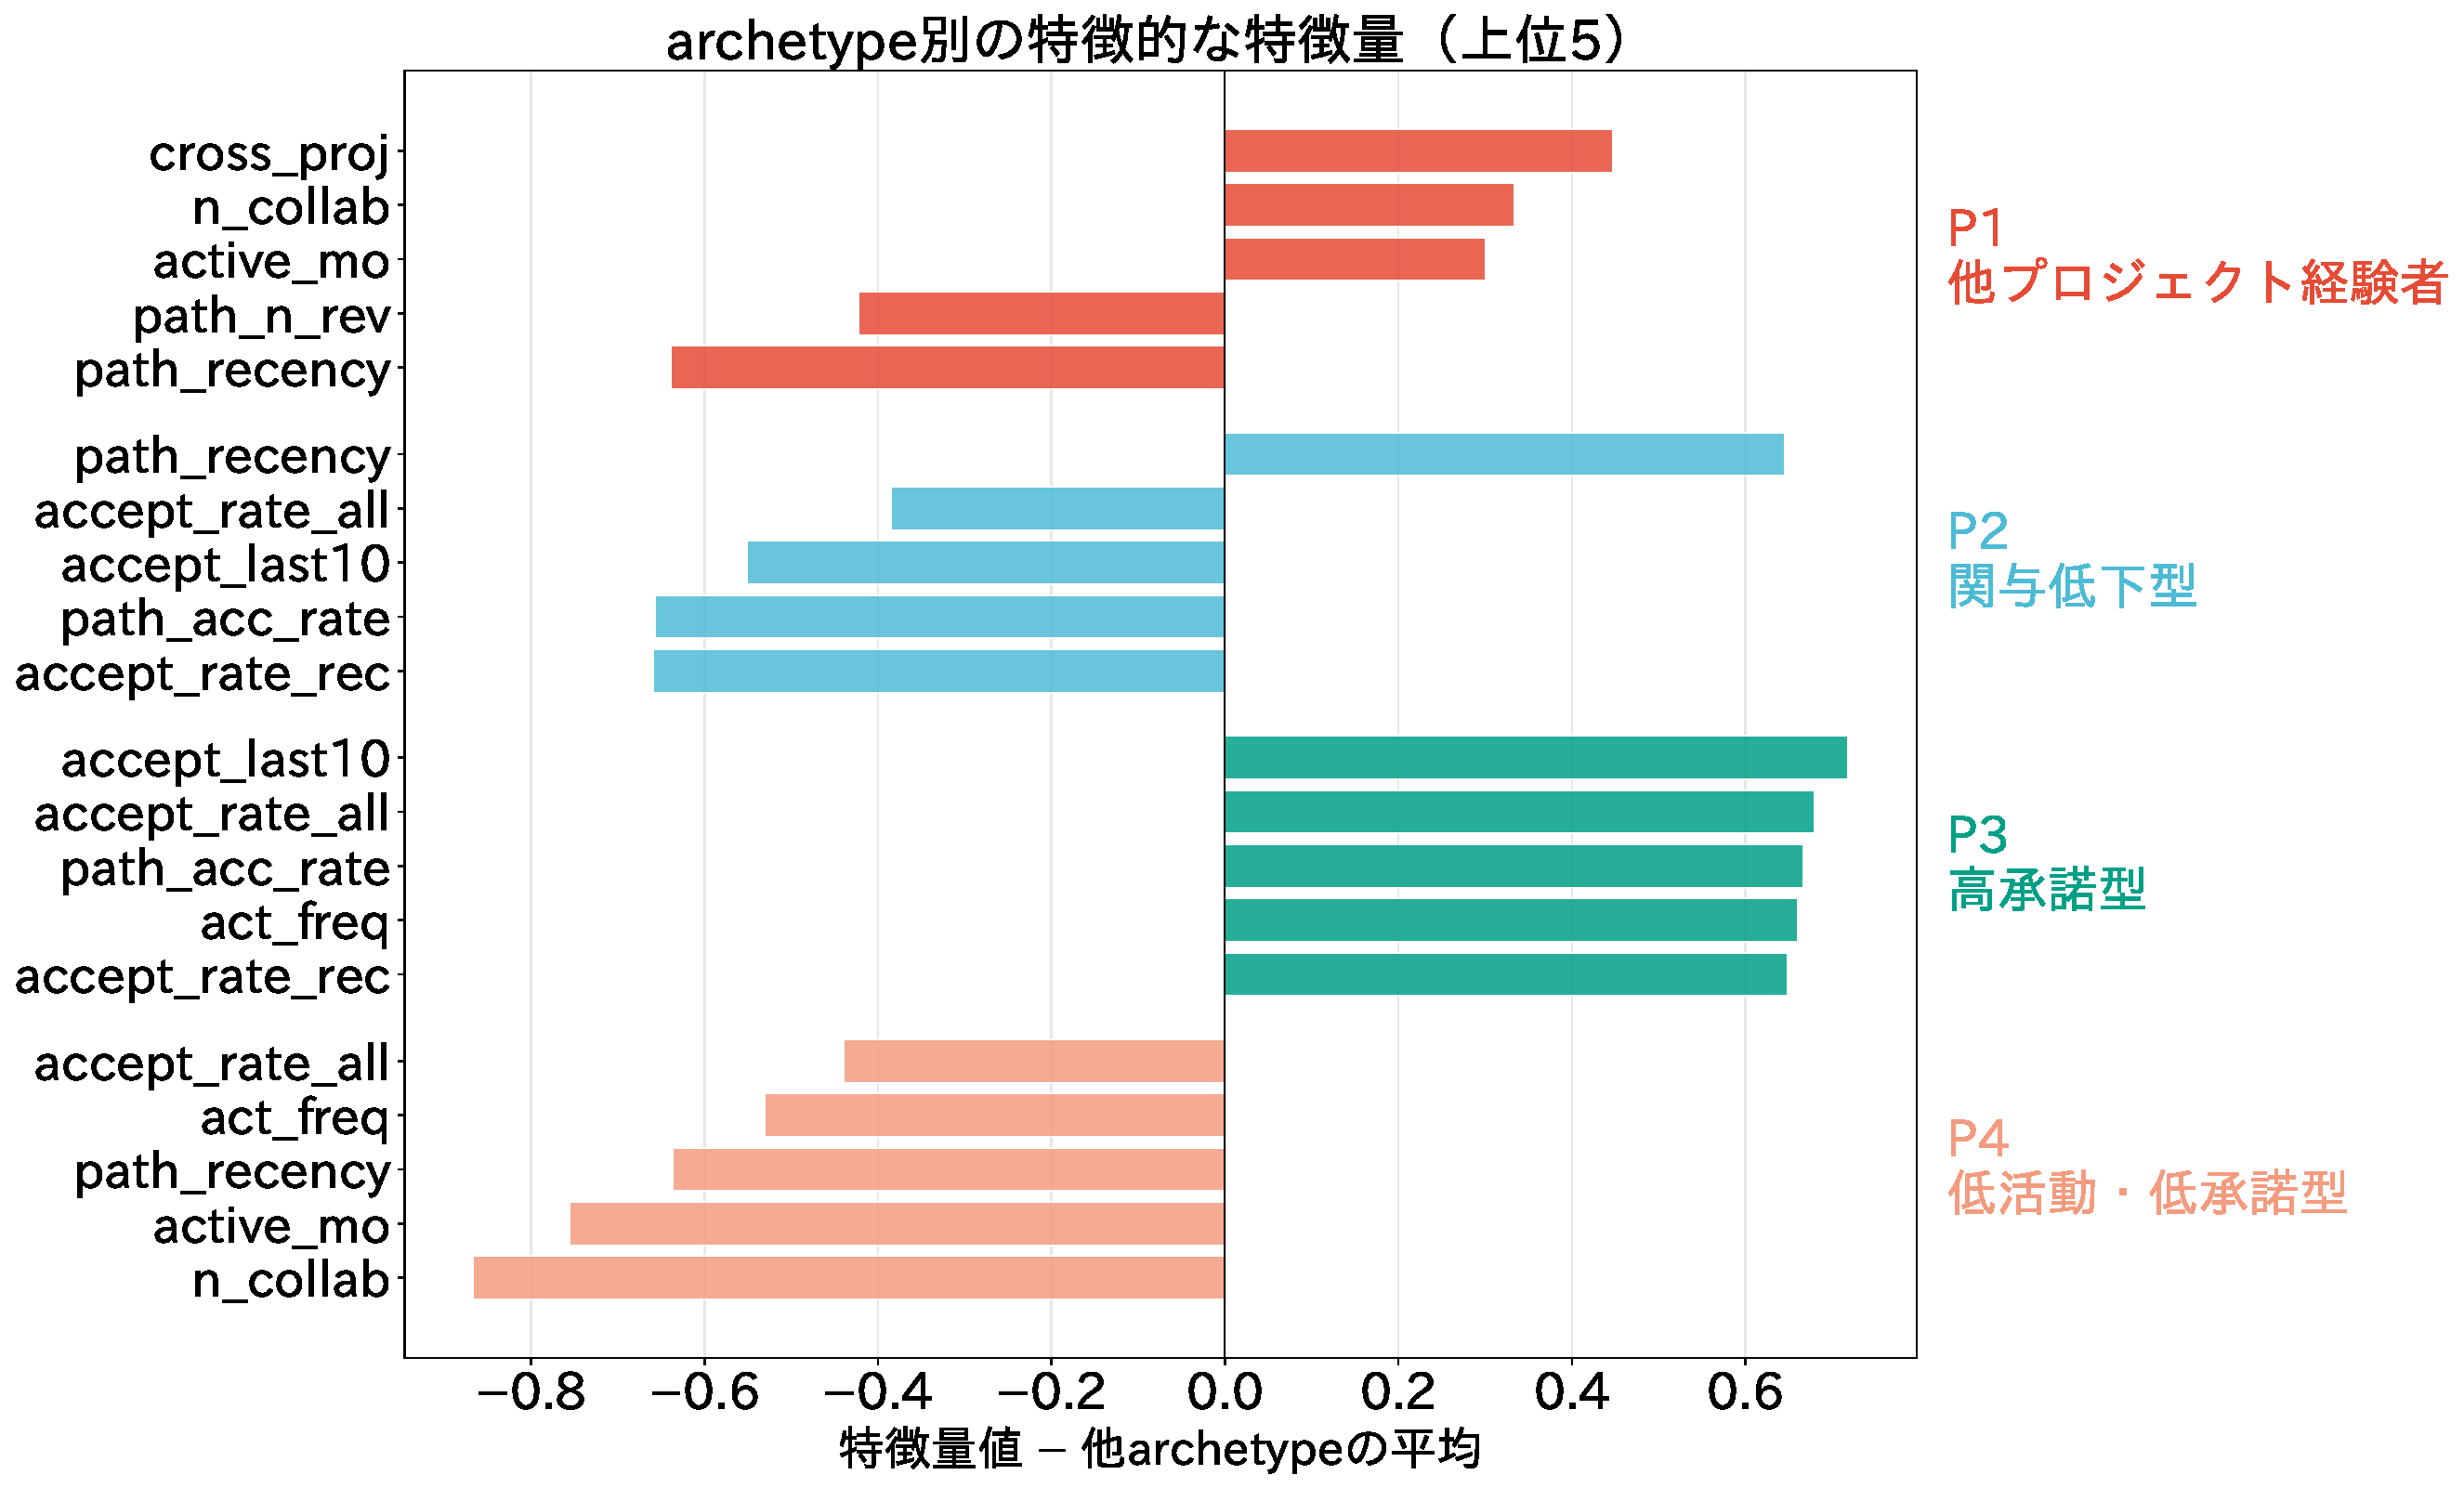
\includegraphics[width=\linewidth]{fig/fig_pair_archetype_profile.pdf}
%   \caption{4ペアarchetypeの特徴的な特徴量}
%   \label{fig:pair-profile}
%   \end{figure}

% \vspace{-8mm}

%   \begin{table}[H]
%   \centering
%   \caption{ペア単位の4原型における評価期間別のAUC差（IRL-RF）（pp，$n=3{,}677$）\todo{差し替え}}
%   \label{tab:pair-arch-delta}
%   \small
%   \begin{tabularx}{\linewidth}{l|*{4}{>{\centering\arraybackslash}X}}
%   \hline
%   Arch. ($n$) & 1--3m & 4--6m & 7--9m & 10--12m \\
%   \hline
%   P1 (1,284) & $+5.7$ & $+0.1$ & $+6.9$ & $-1.6$ \\
%   P2 (928) & $-7.6$ & $-6.1$ & $-3.3$ & $-4.9$ \\
%   P3 (539) & $-8.9$ & $-8.9$ & $+1.1$ & $-1.3$ \\
%   P4 (926) & $+4.1$ & $-1.9$ & $-3.9$ & $+2.9$ \\
%   \hline
%   \end{tabularx}
%   \end{table}
% \end{minipage}
% \hfill
% \begin{minipage}[t]{0.48\linewidth}
%   % 左列：開発者単位
%   \begin{table}[H]
%   \centering
%   \caption{4原型の解釈名（$N=289$）}
%   \label{tab:archetypes}
%   \begin{tabularx}{\linewidth}{l|p{1.6cm}|X|r}
%   \hline
%   ID & 名前 & 特徴 & $n$ \\
%   \hline
%   A1 & 低活動型 & \todo{XX}（same\_domain）は高いが，活動頻度（act\_freq）や活動月数（active\_mo）や\todo{XX}（rev/owner) が低い & 59 \\
%   A2 & 短期・レビュー中心型& \todo{XX}（rev/owner）は高いが，活動月数（active\_mo）や承諾率（accept\_rate\_all）が低い & 69 \\
%   A3 & 高承諾・高活動型 & 直近の承諾率（accept\_last10, accept\_rate\_rec）や活動頻度（act\_freq）が高い & 63 \\
%   A4 & 常時活動・低承諾型 & 活動月数（active\_mo）が長いが，承諾率（accept\_rate\_all等）が低い & 98 \\
%   \hline
%   \end{tabularx}
%   \end{table}

% \vspace{-8mm}

%   \begin{figure}[H]
%   \centering
%   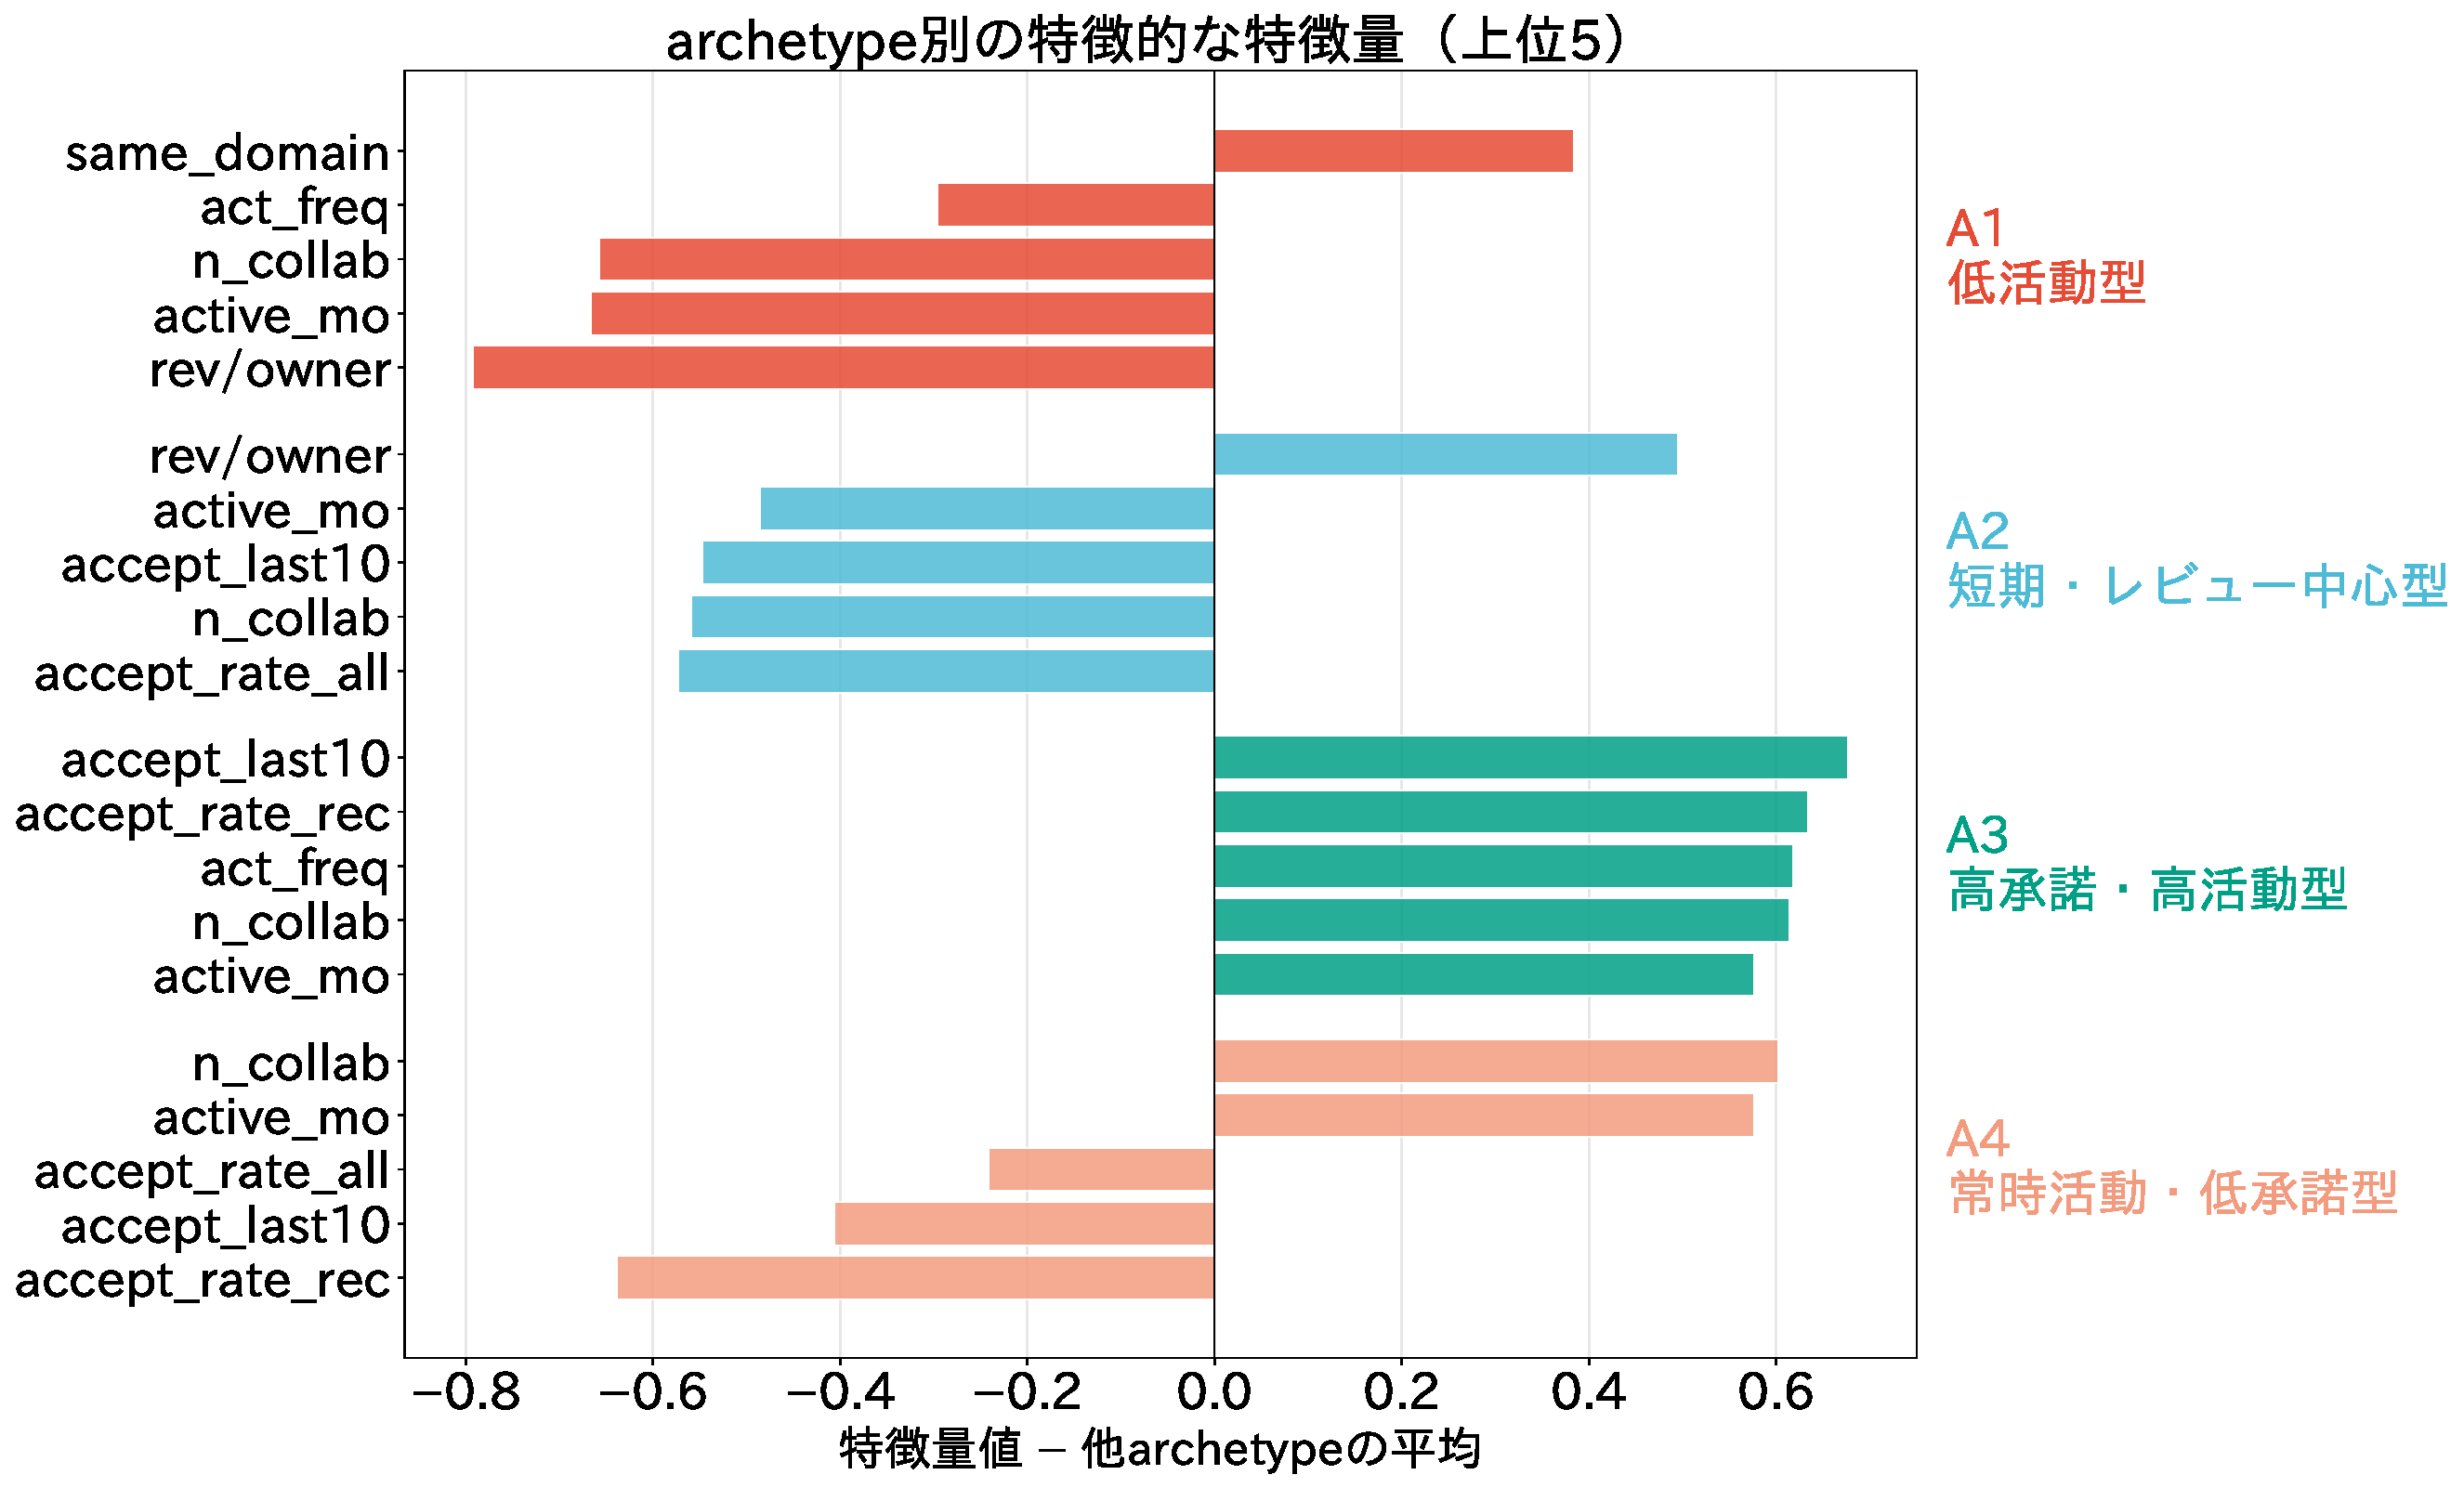
\includegraphics[width=\linewidth]{fig/fig_dev_archetype_profile.pdf}
%   \caption{4開発者archetypeの特徴量プロファイル}
%   \label{fig:dev-profile}
%   \end{figure}

% \vspace{-8mm}

%   \begin{table}[H]
%   \centering
%   \caption{開発者単位の4原型における評価期間別のAUC差（IRL-RF）\todo{差し替え}}
%   \label{tab:dev-arch}
%   \small
%   \begin{tabularx}{\linewidth}{l|*{4}{>{\centering\arraybackslash}X}}
%   \hline
%   Arch. ($n$) & 1--3m & 4--6m & 7--9m & 10--12m \\
%   \hline
%   A1 (341) & $-11.3$ & $-12.3$ & $-6.9$ & $-5.6$ \\
%   A2 (554) & $+1.2$ & $+3.9$ & $+2.1$ & $+5.6$ \\
%   A3 (1,213) & $+2.1$ & $-6.1$ & $-0.9$ & $-2.2$ \\
%   A4 (1,639) & $-3.3$ & $-4.3$ & $+0.2$ & $-0.4$ \\
%   \hline
%   \end{tabularx}
%   \end{table}
% \end{minipage}

% \end{figure*}



\begin{figure*}[t]
\centering
\begin{minipage}[t]{0.48\linewidth}
  % 左列：ペア単位
  \begin{table}[H]
  \centering
  \caption{4 ペアarchetype の解釈名（$n=3{,}677$）}
  \label{tab:pair-arch}
  \begin{tabularx}{\linewidth}{l|p{1.5cm}|X|r}
  \hline
  ID & 名前 & 特徴 & $n$ \\
  \hline
  P1 & 他プロジェクト経験者 & 他プロジェクトへの貢献経験（cross\_proj）を有し，最終活動からの経過時間（path\_recency）が短く，ディレクトリへの過去レビュー数（path\_n\_rev）は少ない & 1{,}284 \\
  P2 & 関与低下型 & 当該ディレクトリの最終活動からの経過時間（path\_recency）が長い & 928 \\
  &&&\\
  P3 & 高承諾型 & 承諾率（accept\_rate\_all等）が高く， & 539 \\
  &&&\\
  P4 & 低活動・低承諾型 & 全体承諾率（accept\_rate\_all）が低く，活動頻度（act\_freq）も少ない & 926 \\
  \hline
  \end{tabularx}
  \end{table}

\vspace{-10mm}

  \begin{figure}[H]
  \centering
  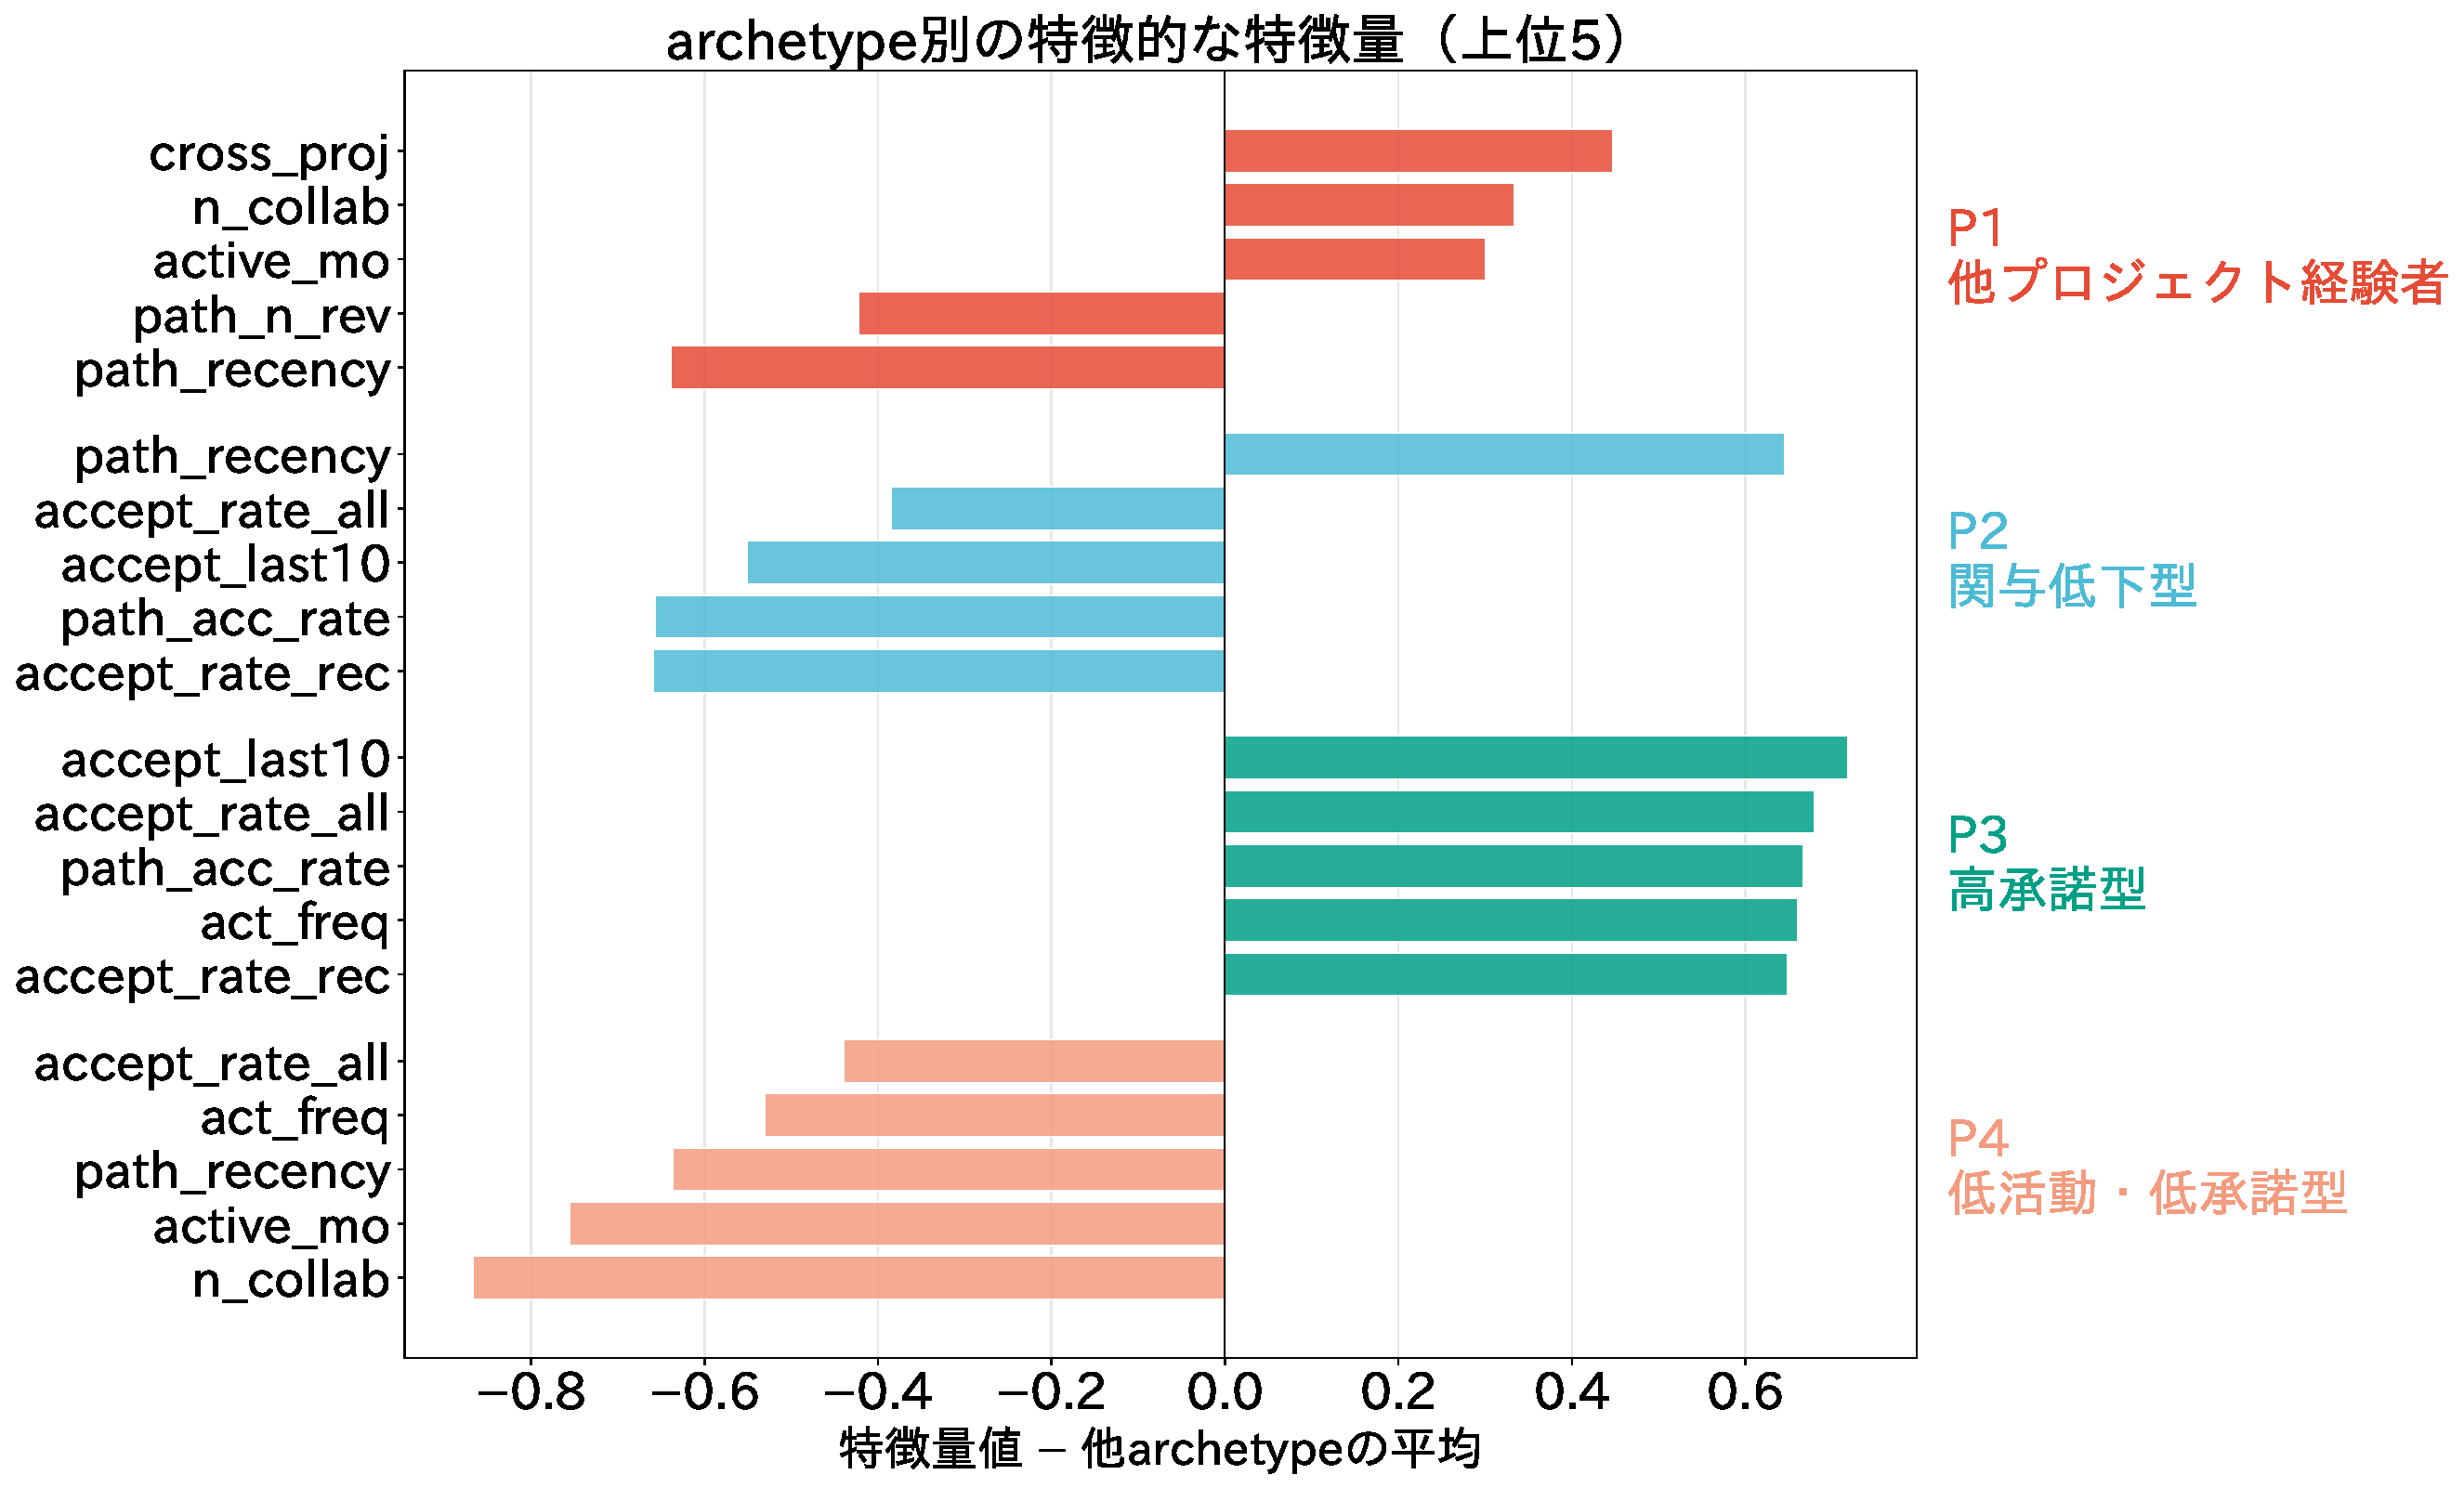
\includegraphics[width=\linewidth]{fig/fig_pair_archetype_profile.pdf}
  \caption{ペア単位の原型分析における特徴的な特徴量}
  \label{fig:pair-profile}
  \end{figure}

\vspace{-10mm}

  \begin{table}[H]
  \centering
  \caption{ペア単位の4原型における評価期間別AUC}
  \label{tab:pair-arch-delta}
  \footnotesize\setlength{\tabcolsep}{4pt}
  \begin{tabularx}{\linewidth}{l|l|*{4}{>{\centering\arraybackslash}X}|>{\centering\arraybackslash}X}
  \hline
  \multicolumn{2}{c|}{} & 1--3m & 4--6m & 7--9m & 10--12m & $\Sigma\Delta$ \\
  \hline
  \multirow{3}{*}{P1 (1,284)} & IRL & 0.765 & 0.742 & 0.706 & 0.654 & \\
   & RF  & 0.675 & 0.703 & 0.664 & 0.708 & \\
   & $\Delta$ & $+9.0$ & $+3.9$ & $+4.2$ & $-5.4$ & $\mathbf{+11.7}$ \\
  \hline
  \multirow{3}{*}{P2 (928)} & IRL & 0.745 & 0.783 & 0.724 & 0.716 & \\
   & RF  & 0.726 & 0.798 & 0.725 & 0.758 & \\
   & $\Delta$ & $+2.0$ & $-1.5$ & $-0.1$ & $-4.2$ & $-3.8$ \\
  \hline
  \multirow{3}{*}{P3 (539)} & IRL & 0.800 & 0.714 & 0.659 & 0.752 & \\
   & RF  & 0.742 & 0.737 & 0.729 & 0.759 & \\
   & $\Delta$ & $+5.8$ & $-2.3$ & $-7.0$ & $-0.7$ & $-4.2$ \\
  \hline
  \multirow{3}{*}{P4 (926)} & IRL & 0.692 & 0.682 & 0.643 & 0.630 & \\
   & RF  & 0.696 & 0.687 & 0.730 & 0.688 & \\
   & $\Delta$ & $-0.4$ & $-0.5$ & $-8.7$ & $-5.9$ & $-15.5$ \\
  \hline
  \end{tabularx}
  \end{table}
\vspace{-6mm}  
\end{minipage}
\hfill
\begin{minipage}[t]{0.48\linewidth}
  % 右列：開発者単位
  \begin{table}[H]
  \centering
  \caption{4原型の解釈名（$N=289$）}
  \label{tab:archetypes}
  \begin{tabularx}{\linewidth}{l|p{1.6cm}|X|r}
  \hline
  ID & 名前 & 特徴 & $n$ \\
  \hline
  A1 & 低活動型 & 活動頻度（act\_freq）・活動月数（active\_mo）・ コード作成に対するレビュー比率（rev/owner）が低く，同一組織からの依頼が多い（same\_domain） & 59 \\
  A2 & 短期・レビュー中心型& \ コード作成に対するレビュー貢献率（rev/owner）が高く，活動月数（active\_mo）や承諾率（accept\_rate\_all）が低い & 69 \\
  A3 & 高承諾・高活動型 & 直近の承諾率（accept\_last10, accept\_rate\_rec）や活動頻度（act\_freq）が高い & 63 \\
  A4 & 常時活動・低承諾型 & 活動月数（active\_mo）が長いが，承諾率（accept\_rate\_all等）が低い & 98 \\
  \hline
  \end{tabularx}
  \end{table}

\vspace{-10mm}

  \begin{figure}[H]
  \centering
  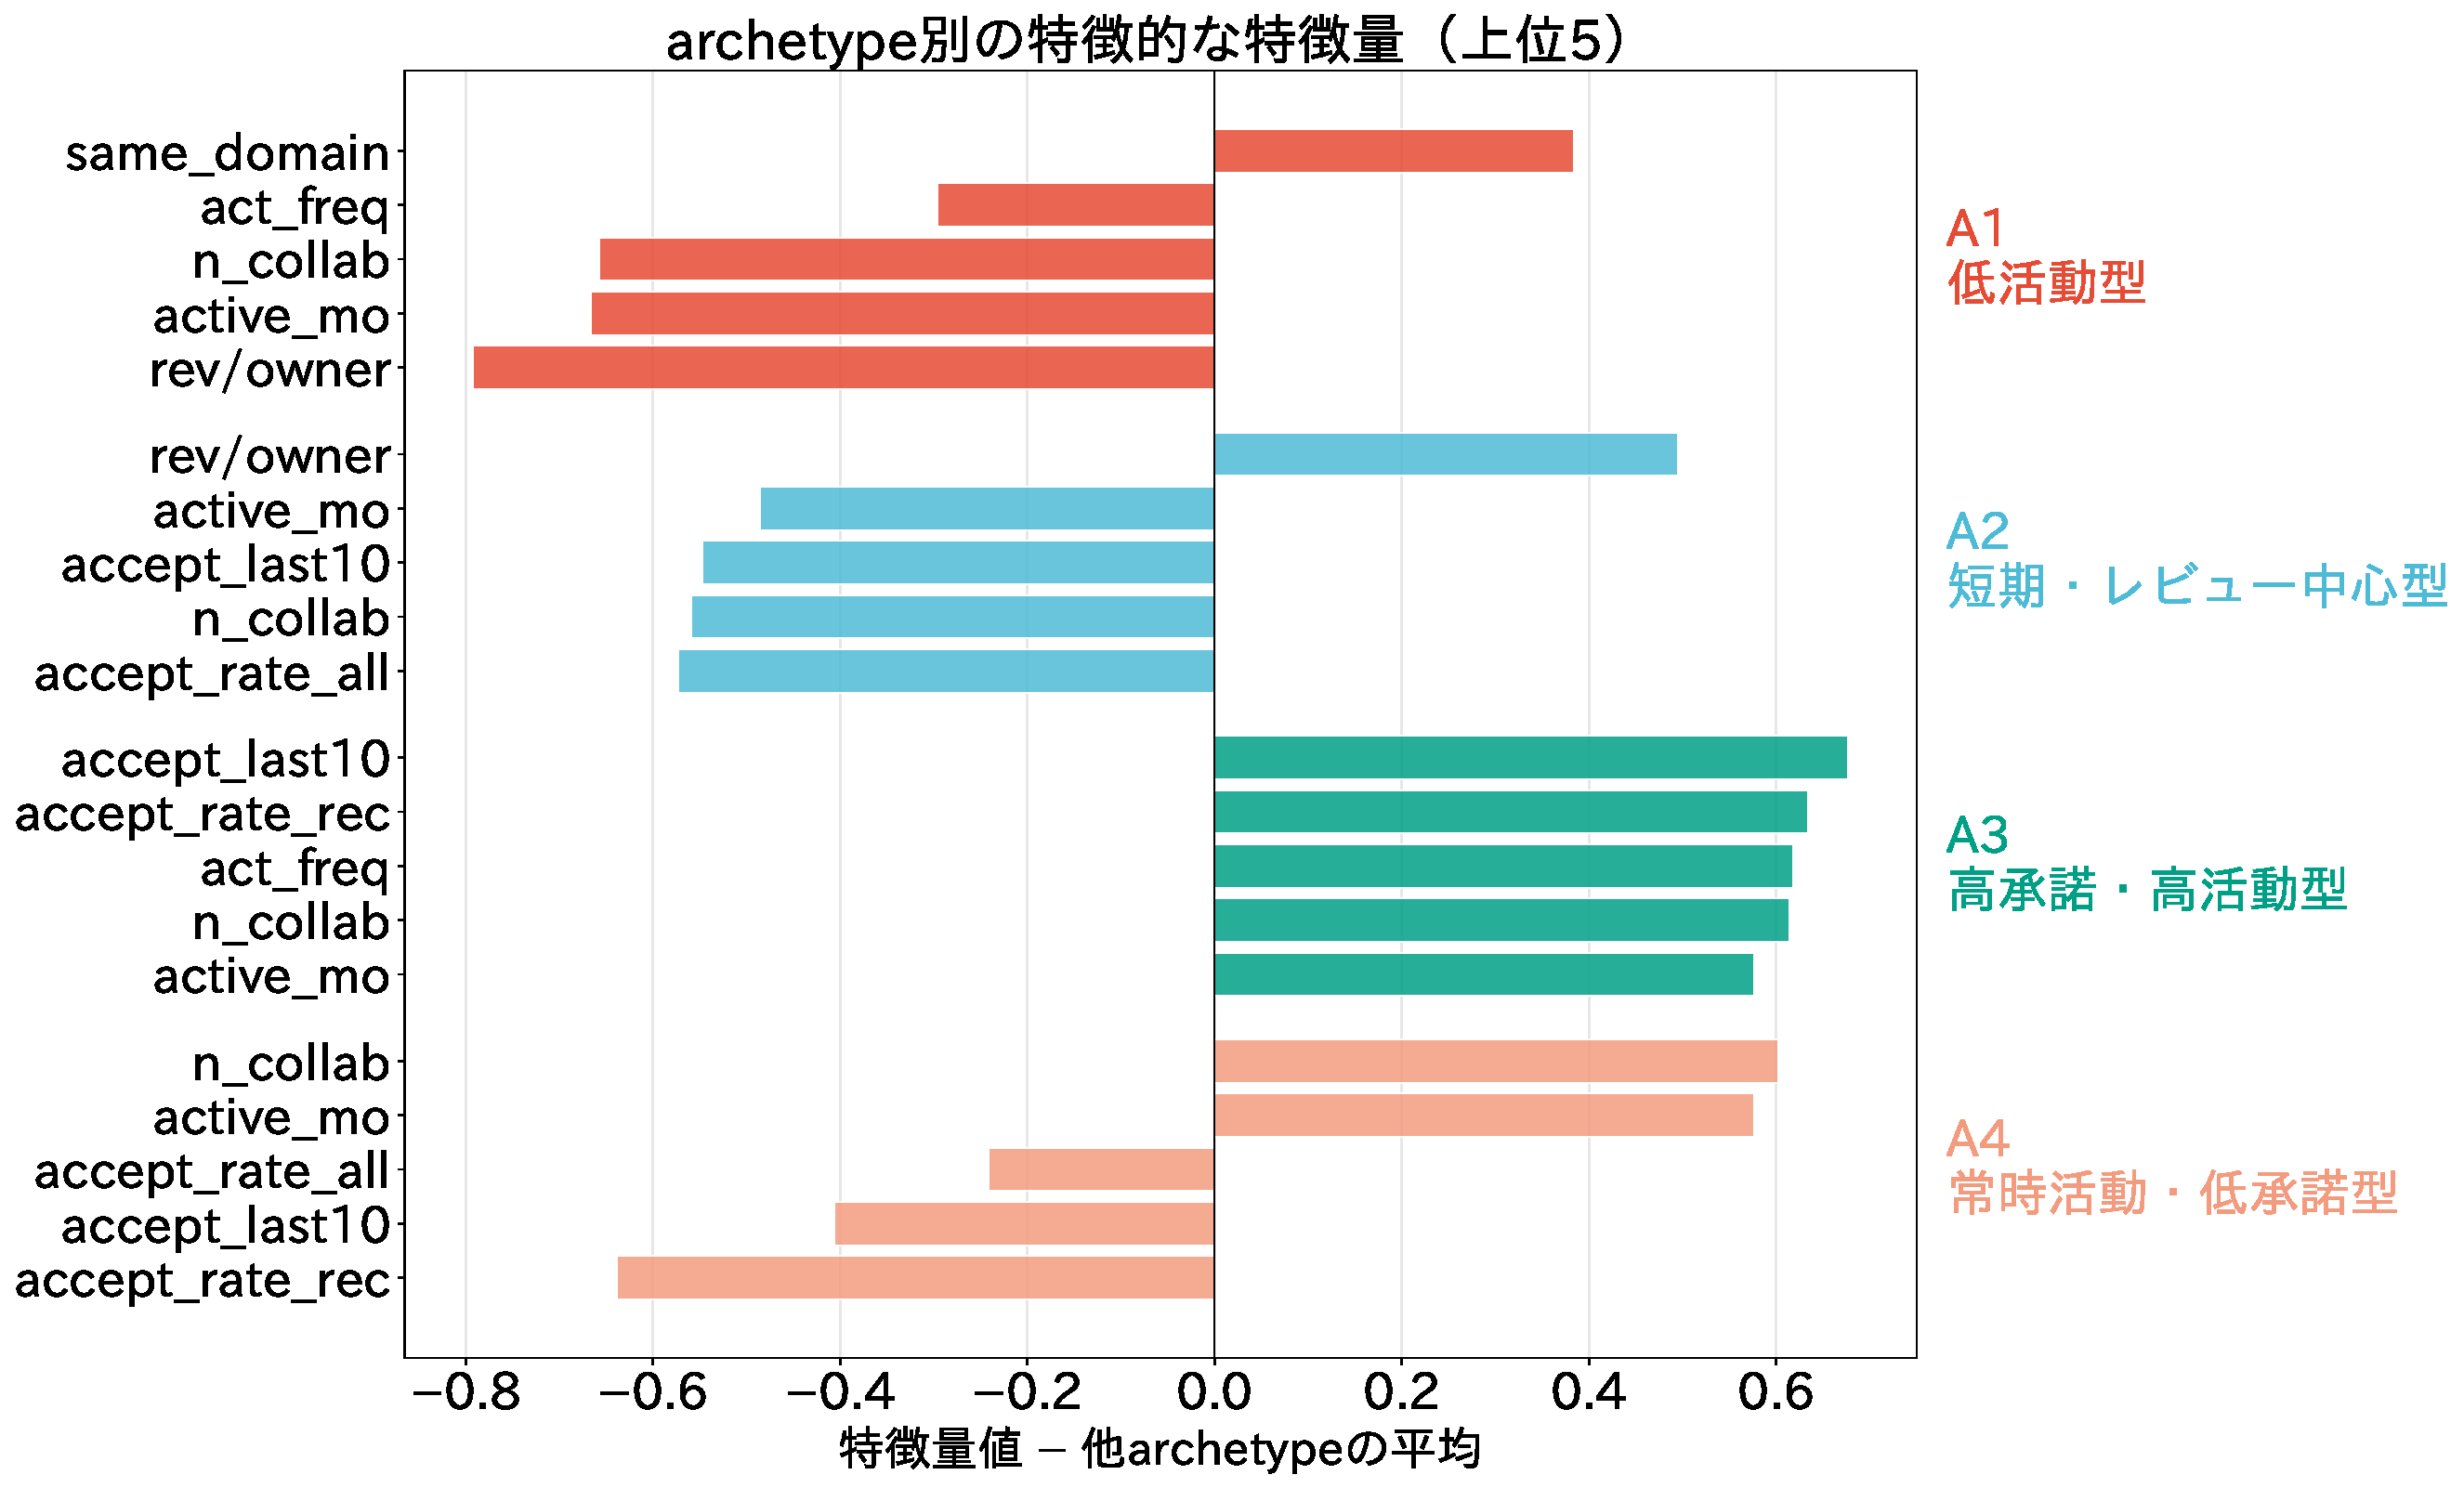
\includegraphics[width=\linewidth]{fig/fig_dev_archetype_profile.pdf}
  \caption{開発者単位の原型分析における特徴的な特徴量}
  \label{fig:dev-profile}
  \end{figure}

\vspace{-10mm}

  \begin{table}[H]
  \centering
  \caption{開発者単位の4原型における評価期間別AUC}
  \label{tab:dev-arch}
  \footnotesize\setlength{\tabcolsep}{4pt}
  \begin{tabularx}{\linewidth}{l|l|*{4}{>{\centering\arraybackslash}X}|>{\centering\arraybackslash}X}
  \hline
  \multicolumn{2}{c|}{} & 1--3m & 4--6m & 7--9m & 10--12m & $\Sigma\Delta$ \\
  \hline
  \multirow{3}{*}{A1 (341)} & IRL & 0.607 & 0.423 & 0.630 & 0.492 & \\
   & RF  & 0.606 & 0.631 & 0.651 & 0.597 & \\
   & $\Delta$ & $+0.1$ & $-20.8$ & $-2.1$ & $-10.5$ & $-33.3$ \\
  \hline
  \multirow{3}{*}{A2 (554)} & IRL & 0.750 & 0.806 & 0.667 & 0.664 & \\
   & RF  & 0.798 & 0.718 & 0.756 & 0.502 & \\
   & $\Delta$ & $-4.9$ & $+8.9$ & $-8.9$ & $+16.2$ & $\mathbf{+11.3}$ \\
  \hline
  \multirow{3}{*}{A3 (1,213)} & IRL & 0.835 & 0.781 & 0.693 & 0.730 & \\
   & RF  & 0.760 & 0.782 & 0.741 & 0.796 & \\
   & $\Delta$ & $+7.5$ & $-0.1$ & $-4.8$ & $-6.5$ & $-3.9$ \\
  \hline
  \multirow{3}{*}{A4 (1,639)} & IRL & 0.791 & 0.832 & 0.763 & 0.773 & \\
   & RF  & 0.746 & 0.814 & 0.747 & 0.793 & \\
   & $\Delta$ & $+4.5$ & $+1.8$ & $+1.6$ & $-2.0$ & $\mathbf{+5.9}$ \\
  \hline
  \end{tabularx}
  \end{table}
\vspace{-6mm} 
\end{minipage}

\end{figure*}

\subsubsection{開発者単位の分析}\label{sec:dev-arch}
開発者単位の原型分析では，ペア単位とは異なり，ディレクトリとの関係性を考慮せず，開発者個別の活動特性に基づき分類する．特徴量は表\ref{tab:features}から，ディレクトリと活動特徴のカテゴリを除く26個の特徴量を用いる．
% 図~\ref{fig:rss}(b)により$K = 4$を採用し，
表~\ref{tab:archetypes}と図~\ref{fig:dev-profile}は，原型分析によって設定した4つの原型の解釈名，および，それぞれの原型の特徴量の分布を示す．表~\ref{tab:dev-arch}に開発者単位の4原型における評価期間別のAUC差（IRL$-$RF）を示す．

A1（低活動型）は，1--3か月はほぼ互角（$+0.1$ pp）だが，それ以降の期間はRFの方が精度が高く，活動履歴が少ない開発者に対しては累積統計量を用いたRFが概ね優位である．
一方，A2（短期・レビュー中心型）では4--6か月（$+8.9$ pp）や10--12か月（$+16.2$ pp）でIRLが上回る期間が見られるが，1--3か月と7--9か月はRFが優位となり，評価期間によって優劣が混在する．
A3（高承諾・高活動型）では1--3か月はIRLが上回るが（$+7.5$ pp），中長期はRFが優位であった（4期間の合計差$-3.9$ pp）．直近の行動変化を捉えるIRLは短期予測に有効だが，中長期では一時的な変動が平均化され，安定した累積承諾実績を用いるRFが優位になると考える．
A4（常時活動・低承諾型）は4期間中3期間でIRLが上回る（$\Sigma\Delta = +5.9$）．訓練期間全体を通じて活動月数（active\_mo）が多いため，長い活動軌跡がIRLの学習を支えると考えられる．
したがって，活動履歴が少ない開発者には累積統計量を用いたRFが有用であり，承諾パターンが不安定な開発者や活動軌跡が長い開発者ではIRLが補完的に働く場合があることを示した．


% \subsubsection{開発者単位の原型}
% 得られた4原型の解釈名を表\ref{tab:archetypes}に，特徴量プロファイルを図\ref{fig:dev-profile}に示す．

% \begin{table}[H]
% \centering
% \caption{4原型の解釈名（$N=289$）}
% \label{tab:archetypes}
% \begin{tabularx}{\linewidth}{l|l|X|r}
% \hline
% ID & 名前 & 特徴 & $n$ \\
% \hline
% A1 & 低活動型 & 履歴薄く直近性低い新参者 & 59 \\
% A2 & 短期・レビュー中心型& PR投稿乏しくレビュー専従度高い & 69 \\
% A3 & 高承諾・高活動型 & 高コラボレータ数・高承諾率の安定層 & 63 \\
% A4 & 常時活動・低承諾型 & 常時活動だが直近承諾率は低めの層 & 98 \\
% \hline
% \end{tabularx}
% \end{table}

% \begin{figure}[H]
% \centering
% 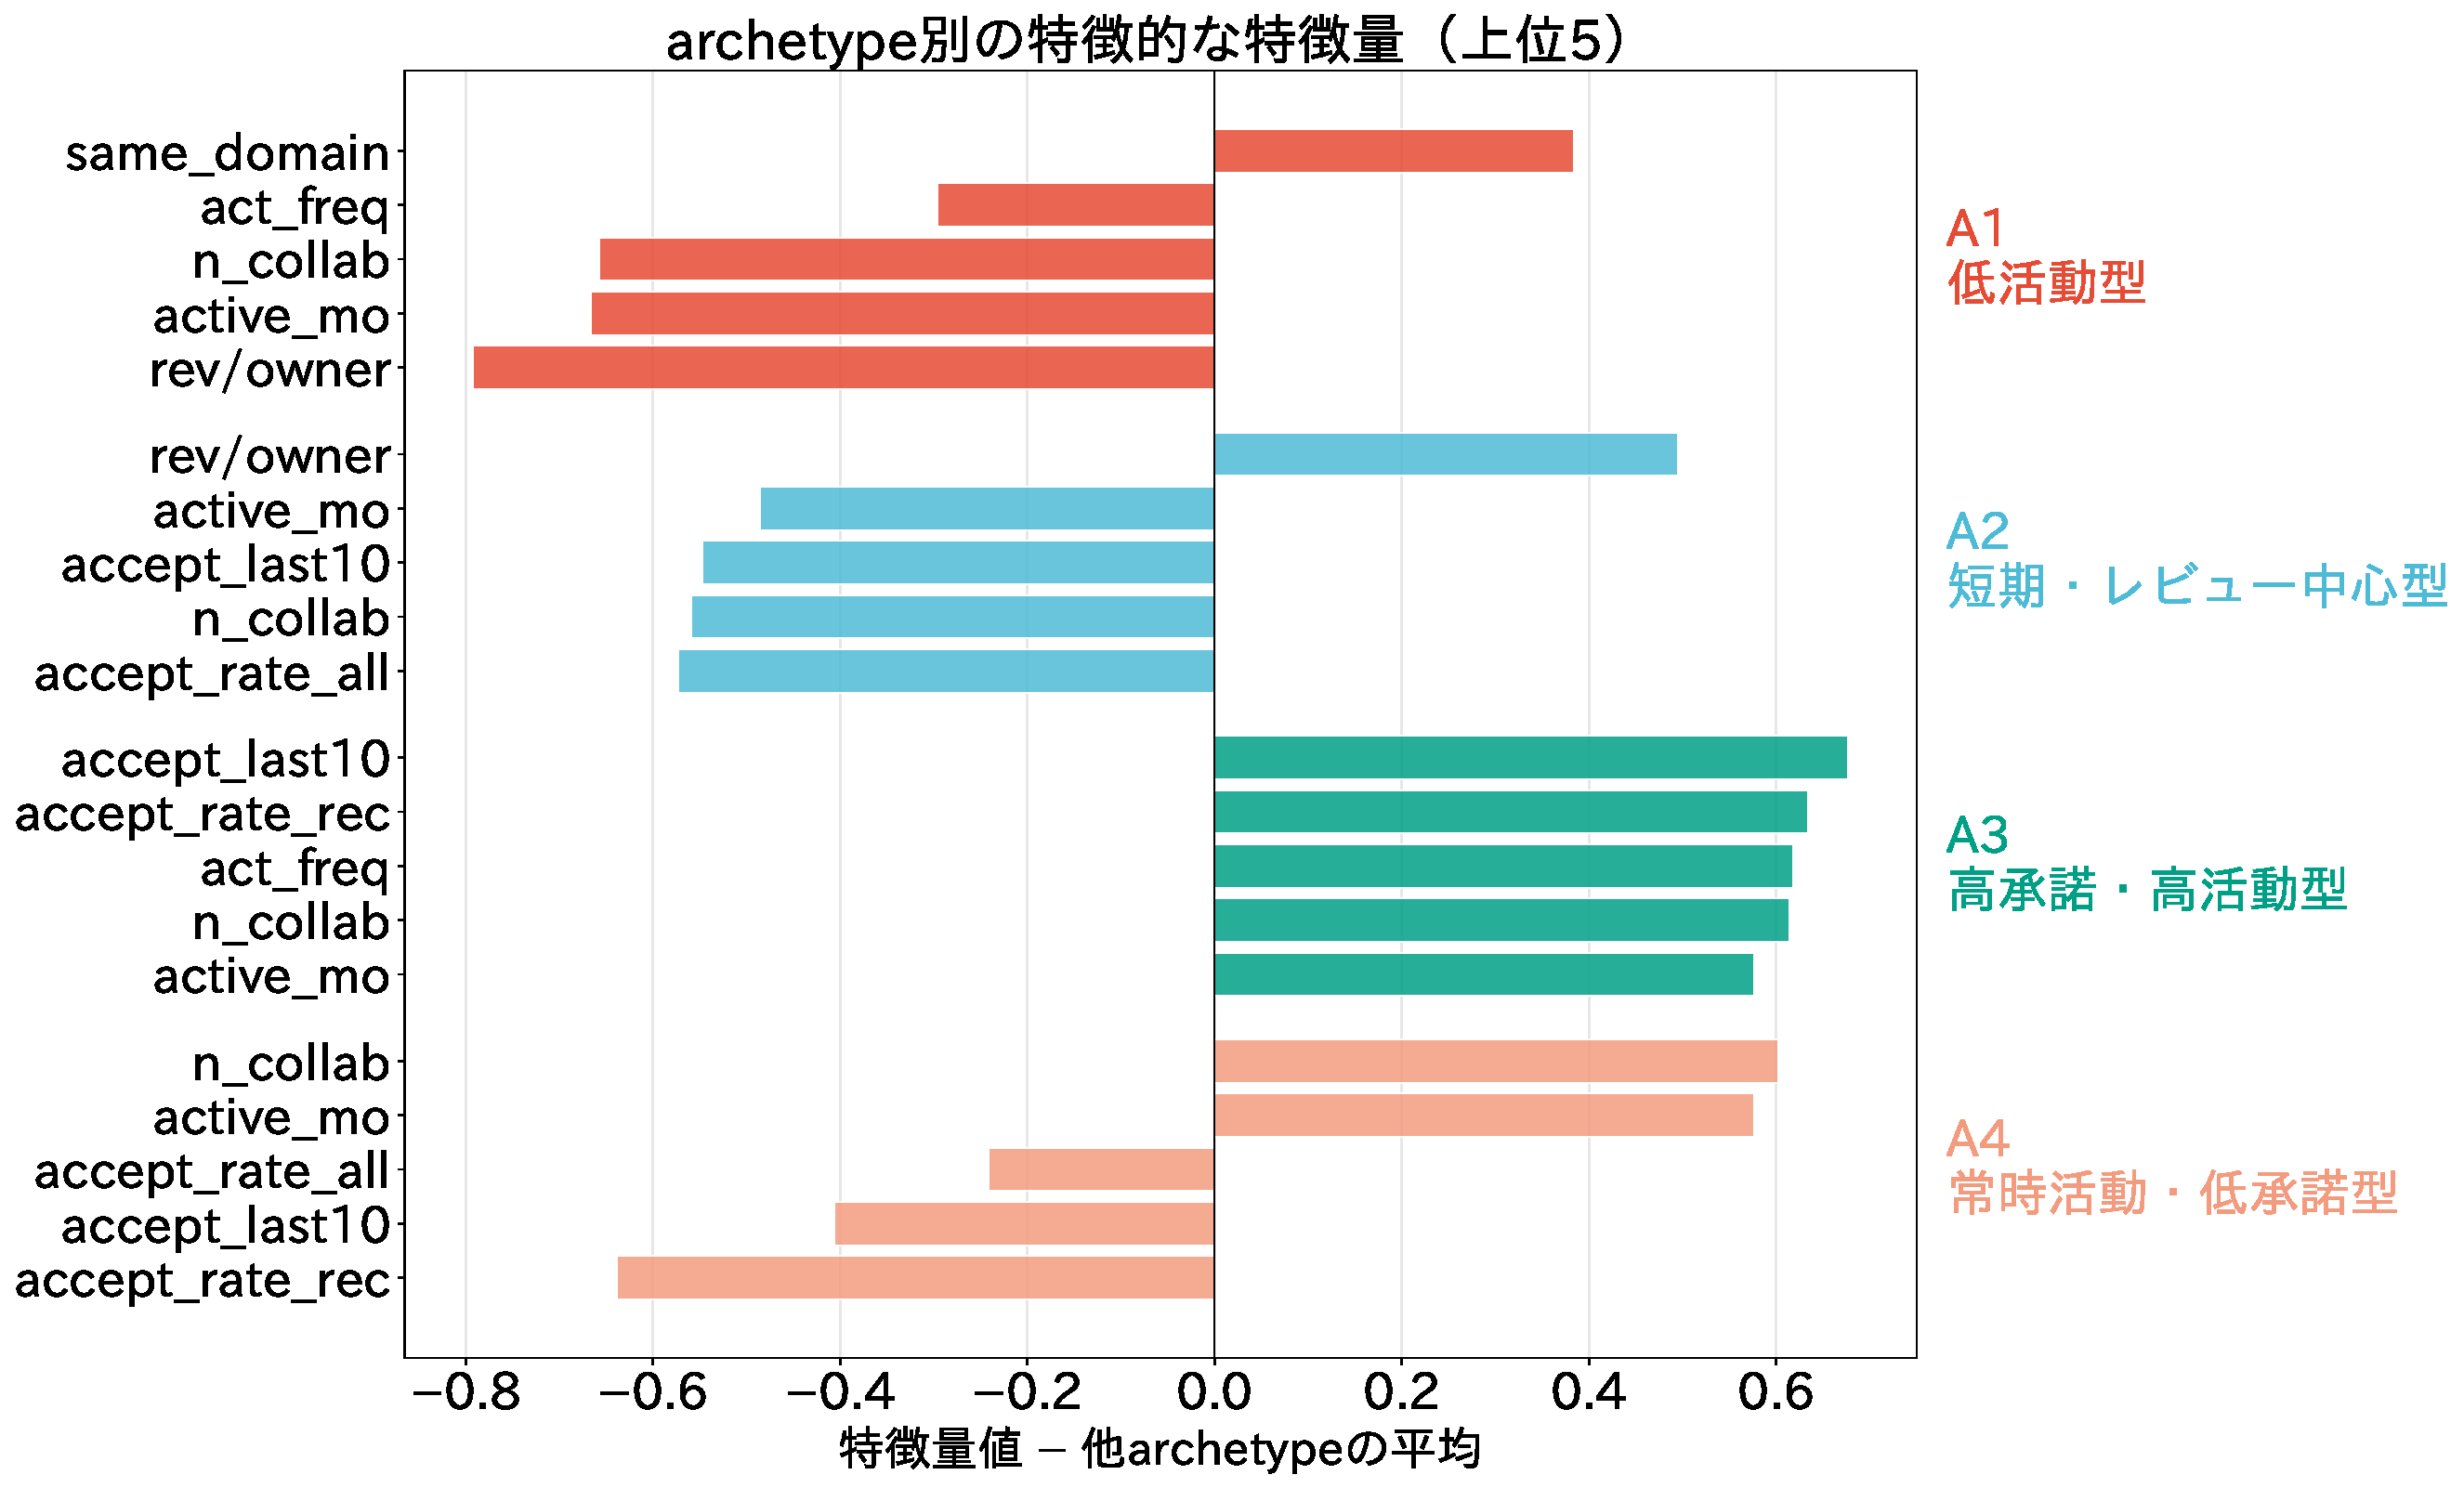
\includegraphics[width=\linewidth]{fig/fig_dev_archetype_profile.pdf}
% \caption{4 開発者archetypeの特徴量プロファイル（Eugster流）．}
% \label{fig:dev-profile}
% \end{figure}

% \subsubsection{開発者タイプ別の補完性}\todo
% 表\ref{tab:dev-arch}に開発者archetype $\times$ 評価期間のAUC差（IRL$-$RF）を示す．A1（低活動型）では全期間でRF優位（最大$-12.3$ pp），A2（短期・レビュー中心型）では全期間でIRL優位（最大$+5.6$ pp）と，4評価期間を跨いだ補完性が確認される．

%----------------------
% \begin{table}[t]
% \centering
% \caption{開発者archetype $\times$ 評価期間のAUC差 IRL$-$RF（pp）\todo{差し替え}}
% \label{tab:dev-arch}
% \small
% \begin{tabularx}{\linewidth}{l|*{4}{>{\centering\arraybackslash}X}}
% \hline
% Arch. ($n$) & 1--3m & 4--6m & 7--9m & 10--12m \\
% \hline
% A1 (341) & $-11.3$ & $-12.3$ & $-6.9$ & $-5.6$ \\
% A2 (554) & $+1.2$ & $+3.9$ & $+2.1$ & $+5.6$ \\
% A3 (1,213) & $+2.1$ & $-6.1$ & $-0.9$ & $-2.2$ \\
% A4 (1,639) & $-3.3$ & $-4.3$ & $+0.2$ & $-0.4$ \\
% \hline
% \end{tabularx}
% \end{table}



% 以上より，主指標のAUCでタイプ依存の補完性が確認された．



% ===== 査読対応 A-2/B-3 ここから =====
\fixstart
\subsection{追加実験：時系列符号化の寄与を分離するアブレーション}\label{sec:ablation}
IRLの精度の源泉が「時系列情報の利用」によるものか，「IRLとしての報酬関数の定式化」によるものかを切り分けるため，同一のバックボーン（LSTM，隠れ層次元128）・同一の特徴量・同一の学習データを用い，教師信号の粒度のみを変えた退化版との比較実験を行った．提案するIRLは行動軌跡の各時点（月次）の行動を教師信号として学習するのに対し，退化版は軌跡の最終時点の行動のみを教師信号とする（全時点教師 vs 最終時点教師のみ）．同様の退化版をGRU・Transformerでも構築し比較した．

表\ref{tab:ablation}に4評価期間のpooled AUC-ROCを示す．IRL本体は，LSTM退化版に対し$+3.8$ pp（bootstrap 95\% CI $[+2.9, +4.7]$，$p<0.0005$），GRU退化版に対し$+4.8$ pp（95\% CI $[+3.8, +5.8]$），Transformer退化版に対し$+7.9$ pp（95\% CI $[+6.9, +8.8]$）と有意に上回った．また，退化版はRFに対しても有意に劣った（LSTM退化版 vs RF: $-5.0$ pp，95\% CI $[-5.8, -4.1]$）ことから，時系列モデルであれば精度が高いわけではなく，IRLの軌跡定式化による全時点教師信号の活用が精度向上に寄与していると考えられる．なお，Transformer退化版のpooled値は評価期間間のスコア尺度の不揃いにより低下しており，期間内順位正規化後は$0.743$まで回復する．また，本実験は単一シードによる学習であり，上記の信頼区間はペア抽出によるブートストラップ由来のものでシード分散は含まない．

\begin{table}[t]
\centering
\caption{IRLと退化版（教師信号を最終時点のみに制限したモデル）のpooled AUC-ROC比較}
\label{tab:ablation}
\footnotesize
\begin{tabularx}{\linewidth}{l*{2}{>{\centering\arraybackslash}X}}
\hline
モデル & pooled AUC-ROC & IRL$-$X (pp) \\
\hline
IRL（提案手法） & \textbf{0.789} & --- \\
LSTM退化版 & 0.751 & $+3.8$ \\
GRU退化版 & 0.741 & $+4.8$ \\
Transformer退化版 & 0.710 & $+7.9$ \\
RF & 0.801 & $-1.2$ \\
\hline
\end{tabularx}
\end{table}
\fixend
% ===== 査読対応 A-2/B-3 ここまで =====

\subsection{追加実験：アンサンブルモデル}
5.3節で確認したIRLとRFは，予測可能な開発者とディレクトリのペア，開発者が異なるため，モデル間で補完することで高い精度が期待できる．追加実験として両モデルの貢献確率の単純平均をアンサンブルの予測値とし，予測精度の改善を検証する．改善幅が偶然でないことを確認するために，bootstrap法により95\%信頼区間を算出して判断する．

% \ref{sec:archetype}節で得られる開発者タイプ別の補完性を活用するため，両モデルの予測確率を式(\ref{eq:ens})の通り単純平均で統合する．
% \begin{equation}
% \label{eq:ens}
% \hat{p}_h^{\mathrm{ens}}(d, r) = \frac{1}{2}\left(\hat{p}_h^{\mathrm{irl}}(d, r) + \hat{p}_h^{\mathrm{rf}}(d, r)\right)
% \end{equation}
% 固定重み0.5で追加学習を持たないため，ベースモデルの訓練期間と評価期間を分離する構造が保持されるため，統合段階での時間的なラベルリークは発生しない．

表\ref{tab:rq3}にアンサンブルモデルの結果を示す．全体では最良単独モデル（IRLとRFのうちAUC-ROCが高い方）と比較して$+2.3$ pp（95\% CI $[+1.7, +2.8]$）の改善を確認した．評価期間別では短中期（1--3, 4--6か月）信頼区間が0を含まない改善が得られたが，長期（7--9, 10--12か月）では改善幅が小さく95\%信頼区間が0を含む．

表~\ref{tab:pair-gain}にペア単位の4原型における評価期間別のアンサンブルモデルの最良単独モデルからの改善精度を示す．ペア単位の4種類（P1，P2，P3，P4）の評価期間別の4種類（合計16種類）のうち，13種類でアンサンブルモデルが最良単独モデルから改善されることを示した（最大$+3.6$ pp，P3 10--12m）．特に，P1（他プロジェクト経験者）は全期間で改善した（$+0.4$〜$+2.2$ pp）．表~\ref{tab:dev-gain}に開発者単位の4原型における評価期間別のアンサンブルモデルの改善幅を示す．A3（高承諾・高活動型）とA4（常時活動・低承諾型）の全期間で正の改善した一方，A1（低活動型）とA2（短期・レビュー中心型）では改善しない期間も確認した．

以上より，ペア数が最も多いP1，開発者数が多いA3・A4は全期間にわたって改善を示したのは，アンサンブルモデルの有効性を示す結果である．本研究では単純平均によるアンサンブルを採用したが，原型や評価期間に応じてモデルを選択する方法を導入することで，さらなる精度改善が期待できる．

%-------------------------
% \begin{table}[t]
% \centering
% % \caption{IRL，RF，アンサンブルによるモデルの精度比較結果と，．CIは$10^3$回のbootstrap（クラス比率維持）による95\%信頼期間．\todo{差し替え}}
% \caption{IRL，RF，アンサンブルによるモデルの精度比較結果と，bootstrapによる95\%信頼期間．\todo{差し替え}}
% \label{tab:rq3}
% \footnotesize
% \setlength{\tabcolsep}{4pt}
% \begin{tabularx}{\linewidth}{l*{4}{>{\centering\arraybackslash}X}l}
% \hline
% 期間 & IRL & RF & アンサンブル & 改善幅 (pp) & 95\% CI \\
% \hline
% 1--3m & 0.779 & 0.792 & 0.813 & $+2.1$ & $[+1.4, +2.8]$ \\
% 4--6m & 0.770 & 0.804 & 0.819 & $+1.5$ & $[+0.8, +2.2]$ \\
% 7--9m & 0.774 & 0.789 & 0.816 & $+2.7$ & $[+2.0, +3.4]$ \\
% 10--12m & 0.779 & 0.793 & 0.815 & $+2.3$ & $[+1.4, +3.2]$ \\
% \hline
% 平均 & 0.775 & 0.794 & \textbf{0.816} & $\mathbf{+2.2}$ & --- \\
% \hline
% \end{tabularx}

% % \centering
% % % \caption{ペアarchetype $\times$ 評価期間のアンサンブル gain vs 最良単独モデル（pp，$n=3{,}677$）\todo{差し替え}}
% % \caption{ペア単位の4原型におけるアンサンブルモデルを用いた評価期間別のAUC差\todo{差し替え}}
% % \label{tab:pair-gain}
% % \footnotesize
% % \setlength{\tabcolsep}{4pt}
% % \begin{tabularx}{\linewidth}{l|*{4}{>{\centering\arraybackslash}X}l}
% % \hline
% % Pair Arch. ($n$) & 1--3m & 4--6m & 7--9m & 10--12m & 平均\\
% % \hline
% % P1 (1{,}284) & $+5.5$ & $+7.3$ & $+2.7$ & $+9.8$ &\\
% % P2 (928) & $+2.6$ & $+2.4$ & $+1.6$ & $+3.3$ &\\
% % P3 (539) & $+0.6$ & $+4.1$ & $+8.5$ & $+6.0$ &\\
% % P4 (926) & $+9.9$ & $+5.5$ & $+5.5$ & $+13.0$ &\\
% % \hline
% % ALL (3{,}677) & $+6.4$ & $+4.4$ & $+5.5$ & $+5.7$ &\\
% % \hline
% % \end{tabularx}

% % \centering
% % % \caption{開発者archetype $\times$ 評価期間のアンサンブル gain vs 最良単独モデル（pp，$n=3{,}677$）\todo{差し替え}}
% % \caption{開発者単位の4原型におけるアンサンブルモデルを用いた評価期間別のAUC差\todo{差し替え}}
% % \label{tab:pair-gain}
% % \footnotesize
% % \setlength{\tabcolsep}{4pt}
% % \begin{tabularx}{\linewidth}{l|*{4}{>{\centering\arraybackslash}X}l}
% % \hline
% % Developer Arch. ($n$) & 1--3m & 4--6m & 7--9m & 10--12m & 平均\\
% % \hline
% % A1&&&&&\\
% % A2&&&&&\\
% % A3&&&&&\\
% % A4&&&&&\\
% % \hline
% % ALL (XX) &&&&&\\
% % \hline
% % \end{tabularx}
% % \end{table}
% % %-------------------------

\begin{table}[t]
\centering
\caption{IRL，RF，アンサンブルによるモデルの精度比較結果と，bootstrapによる95\%信頼区間．}
\label{tab:rq3}
\footnotesize
\setlength{\tabcolsep}{4pt}
\begin{tabularx}{\linewidth}{l*{4}{>{\centering\arraybackslash}X}l}
\hline
期間 & IRL & RF & アンサンブル & 改善幅 (pp) & 95\% CI \\
\hline
1--3m & 0.826 & 0.791 & 0.838 & $+1.2$ & $[+0.8, +1.8]$ \\
4--6m & 0.813 & 0.812 & 0.842 & $+2.9$ & $[+2.3, +3.6]$ \\
7--9m & 0.751 & 0.792 & 0.799 & $+0.6$ & $[-0.5, +1.7]$ \\
10--12m & 0.754 & 0.806 & 0.808 & $+0.2$ & $[-0.7, +1.3]$ \\
\hline
全体 & 0.789 & 0.801 & \textbf{0.823} & $\mathbf{+2.3}$ & $[+1.7, +2.8]$ \\
\hline
\end{tabularx}
\vspace{-2mm}
\vspace{1em}

\centering
\caption{ペア単位の4原型におけるアンサンブルモデルを用いた評価期間別のAUC差（アンサンブル$-$最良単独）}
\label{tab:pair-gain}
\footnotesize
\setlength{\tabcolsep}{2pt}
\begin{tabularx}{\linewidth}{p{2.2cm}|*{5}{>{\centering\arraybackslash}X}}
\hline
ペア単位 ($n$) & 1--3m & 4--6m & 7--9m & 10--12m & 合計 \\
\hline
P1 (1,284) & $+0.4$ & $+2.2$ & $+1.7$ & $+1.2$ & $+5.5$ \\
P2 (928)   & $+0.9$ & $+1.3$ & $+1.3$ & $-0.1$ & $+3.4$ \\
P3 (539)   & $+2.5$ & $+0.8$ & $+0.2$ & $+3.6$ & $+7.1$ \\
P4 (926)   & $+2.8$ & $+3.0$ & $-3.3$ & $-1.3$ & $+1.2$ \\
\hline
\end{tabularx}
\vspace{-2mm}
\vspace{1em}

\centering
\caption{開発者単位の4原型におけるアンサンブルモデルを用いた評価期間別のAUC差（アンサンブル$-$最良単独）}
\label{tab:dev-gain}
\footnotesize
\setlength{\tabcolsep}{2pt}
\begin{tabularx}{\linewidth}{p{2.2cm}|*{5}{>{\centering\arraybackslash}X}}
\hline
開発者単位 ($n$) & 1--3m & 4--6m & 7--9m & 10--12m & 合計 \\
\hline
A1 (341)     & $+2.8$ & $-9.3$ & $+1.7$ & $-2.5$ & $-7.3$ \\
A2 (554)     & $+2.0$ & $-0.4$ & $-4.4$ & $-12.6$ & $-15.4$ \\
A3 (1{,}213) & $+1.6$ & $+3.9$ & $+2.1$ & $+0.9$ & $+8.5$ \\
A4 (1{,}639) & $+0.4$ & $+1.7$ & $+1.4$ & $+1.6$ & $+5.1$ \\
\hline
\end{tabularx}
\end{table}


% \subsubsection{開発者単位の評価と統計検定}
% 混合ラベル subset（$N=234$）の開発者別AUC平均はIRL $0.666$ / RF $0.689$ / アンサンブル $0.704$である．paired Wilcoxon符号順位検定（両側）にBonferroni補正（$\times 2$）を適用した結果，開発者別AUCベースで両比較とも有意改善を確認した（Ens vs IRL: $W=7{,}637.5$, $p_{\mathrm{corr}} = 2.7 \times 10^{-7}$, $r = 0.40$；Ens vs RF: $W=10{,}636.5$, $p_{\mathrm{corr}} = 2.3 \times 10^{-2}$, $r = 0.19$）．

% アンサンブルはペア単位で$+2.2$ pp（4評価期間全てで有意），開発者単位でも開発者別AUCに対するWilcoxon検定で有意改善を達成し，追加学習を持たない単純平均でも統計的に頑健な改善が得られることを示した．

% \subsubsection{ペアarchetype 別のアンサンブル効果}\label{sec:pair-gain}
% \ref{sec:pair-arch}節で示した ペアarchetype の補完性が実際に アンサンブル の効きに反映されるかを確認するため，ペアarchetype $\times$ 評価期間のアンサンブル gain（vs 最良単独モデル）を表\ref{tab:pair-gain}に示す．\textbf{16セル全てで正の改善}（$+0.6$〜$+13.0$ pp）であり，特に\textbf{P1（他プロジェクト経験者）と P4（低活動・低承諾型 ）で改善幅が大きい}（最大 +13.0 pp at P4 10--12か月）．これは\ref{sec:pair-arch}節の補完性パターン（P1/P4 でIRL/RFの誤り方向が分岐しやすい）と整合し，補完性が強いセルほどアンサンブルの効きが大きいことを示す．



%%%%%%%%%%%%%%%%%%%%%%%%%
\section{考察}\label{sec:discuss}
%%%%%%%%%%%%%%%%%%%%%%%%%

\subsection{IRLとRFの補完性に関する考察}
5.3節で観察されたモデル間の補完性は，開発者の原型ごとに行動パターンが異なることによる結果と考える．
A1（低活動型）は，貢献数が少なく行動軌跡が短くいため，IRLで開発者の行動パターンを十分に学習できなかったことが考えられる．一方，RFは累積活動量が少ないことが，活動停止を予測する特徴量としてモデルに寄与するため，3か月以降の評価期間ではIRLよりも高い精度で予測できた．1--3か月では
両モデルとも精度が低く大きな差がなかった．

A2（短期・レビュー中心型）では，累積統計量のみを用いるRFは訓練期間の低い承諾率をそのまま反映するため，評価期間の行動変化を捉えることが難しいが，月次の行動軌跡を通じて状態変化を取り込めるIRLは部分的な行動変化を捉えられたと考える．なお，A2ではIRLとRFの優劣が評価期間によって入れ替わっており，これはOpenStackが半年ごとにリリースを行うため，リリースサイクルに伴う活動パターンの変化が影響していることも考えられる．

A3（高承諾・高活動型）では，貢献率が高く，活動も活発で行動パターンが安定しているため，時系列的な変動を考慮せずとも類型統計量を用いるRFが有効であったと考える．ただし，1--3か月ではIRLが優位であった．これは他の期間に比べて直近の活発な行動パターンをIRLがとらえ捉えたことが原因と考える．

A4（常時活動・低承諾型）では，活動月数が多く，行動履歴が豊富なため，両モデルとも安定した精度を示し，優劣の差は小さくなったと考える．
両モデルともアンサンブルの改善幅が全期間で正（A3: $+0.9$〜$+3.9$ pp，A4: $+0.4$〜$+1.7$ pp）となり，両モデルでほぼ同じ精度であった．しかし，IRLが誤予測するペアとRFが誤予測するペアが異なるため，単純平均によるアンサンブルの効果が安定して示された．
開発者の原型とペアの原型で補完性の傾向が異なる．ペアの原型では，貢献経験が少ないペア（P1 他プロジェクト経験者）は特定のディレクトリの累積統計量が少ないため，RFよりもIRLが有効であったと考える．一方で，ディレクトリへの貢献経験を有するペア（P2 関与低下型，P3 高承諾型）では累積統計量が有効に寄与するRFの精度が高くなったと考える．

% ディレクトリ親和度を含むペア単位で見るほうが補完性が鮮明になる事実は，予測単位として開発者-ディレクトリペアを採用した本研究の設計と整合する．

\vspace{-3mm}
\subsection{アンサンブルの有効性に関する考察}
両モデルの予測確率の単純平均が，精度向上につながった理由を考察する．第一に，両モデルが異なる開発者タイプで予測を外していることが考えられる．A1ではRFが概ね優位（最大$-20.8$ pp），A2では一部の評価期間（4--6, 10--12か月）でIRLが優位となる傾向が見られた．このように，IRLの予測結果が誤るペアと，RFの予測結果が誤るペアとが異なるため，単純平均でも誤予測が部分的に相殺され，全体として精度が改善したと考える．

第二に，ペアの原型と評価期間の16通りの組み合わせのうち，13通りでアンサンブルの改善がみられ（最大$+3.6$ pp），特にP1（他プロジェクト経験者）では全期間で改善した．これは\ref{sec:pair-arch}節で示した補完性がアンサンブルの精度改善につながったと考える．

%%%%%%%%%%%%%%%%%%%
\section{妥当性への脅威}\label{sec:validity}
%%%%%%%%%%%%%%%%%%%

\subsection{内的妥当性}
訓練時に評価期間の情報が混入することが懸念されるが，ベースモデルは訓練期間と評価期間を時系列に分離して学習し，未来の情報を学習することがないよう設計している．アンサンブルモデルにおいても，単純平均でるため統合段階で未来の情報を学習することはない．原型分析は評価集合の特徴量から原型と重み$\bm{\alpha}$を計算しているが，補完性の事後解釈にのみ用いておりモデルの訓練・評価とは独立しているためAUCには影響しない．

\subsection{外的妥当性}
評価対象はOpenStackの32の主要プロジェクトに限定しているため，他のOSSプロジェクトに対する結果の一般化に向けた評価は今後の課題とする．GitHubのPull Requestベースのワークフローを採るプロジェクトとは，レビュー単位や承諾の表現粒度が異なることも考えられ，本研究の補完性パターンが他のレビュープラットフォームでも同様に観測されるかは未検証である．ただし，アンサンブルモデルの有効性は，累積統計量を用いるRFと時系列情報を用いるIRLが互いに異なるペアで誤予測するという知見は，他のOSSにおいて同じ補完性が有効であることを期待できる．
スナップショット時刻$t_0$を2023年1月1日に固定しているため，
異なる日時での再現は未検証である．ただし，OpenStackは半年ごとに新バージョンをリリースするため，訓練期間（3年間）および評価期間（1年間）にはリリース前後の活動量の変動が複数回含まれる．
したがって，リリースサイクルに依存した偏りは分析期間内にも存在し，単一の$t_0$であっても分析として結果の信頼性は確保されていると考える．

\section{おわりに}\label{sec:conclusion}
本研究は，特定のモジュールに対して特定の開発者がレビューに貢献するか否かの予測に対し，時系列情報を用いるIRLと累積統計量を用いるRFのモデルを構築した．
ケーススタディとして，OpenStackの公式サービスリポジトリ32件を対象に実験を行った．原型分析で分解した開発者のタイプ間では，両方のモデルは予測結果を補完しあうことで精度向上が期待されることを明らかにし，アンサンブルモデルを提案した．その結果，それぞれのモデルの最大値に比べ，平均$+2.3$ ppの改善が見られた．
今後は，IRLが推定した報酬関数を環境のフィードバックとして組み込み，
開発者の継続性を考慮したレビュー依頼の推薦方策の設計と評価へ展開する．

% 本研究は，OSSレビュアー継続予測に対し，時系列符号化のIRLと累積統計のRandom Forestの補完性に着目したアンサンブルを提案した．OpenStack governance下の32リポジトリ・4評価期間で，両モデルの全体精度は拮抗するもののArchetypal Analysisで分解した開発者タイプ間でIRLとRFには得意領域の補完性が存在し，単純平均のアンサンブルがペア単位で平均$+2.2$ ppの有意な改善を達成することを示した．

% 得られた知見は次の2点である．IRLはRFと単独で競うのではなく補完的に統合することで価値が顕在化すること，固定重み0.5の単純平均は追加学習やハイパーパラメータ調整を要さないため既存のRFベースのパイプラインへ低コストで導入できることである．

% 今後は本研究の継続予測モデルを基盤として，逆強化学習から強化学習への展開に取り組む．具体的には，IRLが推定した報酬関数および活動する確率を環境のフィードバックとして組み込み，レビュー依頼の割り当てを行動とする強化学習エージェントを，開発者の継続性を考慮した推薦方策の最適化として学習する．これにより，継続予測の精度向上にとどまらず，依頼配分を通じてOSSプロジェクト全体の長期的な活動継続を促進する推薦方策の設計と評価へ展開する．また，固定重み0.5の単純平均には限界があるため，archetypeや評価期間に応じた重み付けなどに取り組む．

\vspace{6mm}
\begin{acknowledgment}
本研究はJSPS科研費25K15058の助成を受けたものです．
\end{acknowledgment}
\bibliographystyle{ipsjunsrt}
\bibliography{Hashimoto}

\end{document}

